\documentclass[aspectratio=169,12pt]{beamer}
% ============================================================================
% PROJECT AGORA -- 5 August 2026
% Compile with: latexmk -xelatex project-agora.tex
%
% STRUCTURE:
%   Framing | I Round the world (8 jurisdictions, 2+ slides each)
%   II Agora in detail | III Lineage and rival constitutions
%   IV Swift and competing networks | V Technology | VI Australia (brief)
%   Close | Appendix (not presented)
% Slides marked "% FAST" are 30-45 second glance slides.
%
% SPEAKER NOTES: every frame carries a \note. To render them, uncomment ONE of:
% \setbeameroption{show notes on second screen=right}   % dual-screen (pgfpages)
% \setbeameroption{show notes}                          % interleaved pages
% ============================================================================

\usepackage{fontspec}
\setsansfont{lmsans10-regular.otf}[BoldFont=lmsans10-bold.otf]
\usepackage{microtype}
\usepackage{booktabs}
\usepackage{tabularx}
\usepackage{array}
\usepackage{ragged2e}
\usepackage{graphicx}
\usepackage{tikz}
\usetikzlibrary{arrows.meta}
\usepackage{hyperref}
\usepackage{pgfpages} % required only if a show-notes option above is enabled

\definecolor{Ink}{HTML}{17242D}
\definecolor{Paper}{HTML}{F5F1E8}
\definecolor{Rust}{HTML}{B94E35}
\definecolor{Ocean}{HTML}{2F6B84}
\definecolor{Sage}{HTML}{6D806F}
\definecolor{Gold}{HTML}{B68A3E}
\definecolor{Mist}{HTML}{DDE5E6}
\definecolor{Soft}{HTML}{E9E3D8}
\definecolor{Quiet}{HTML}{5E6B73}
\definecolor{White}{HTML}{FFFFFF}

\hypersetup{colorlinks=true,urlcolor=Ocean,linkcolor=Ink,citecolor=Ocean}

\setbeamercolor{normal text}{fg=Ink,bg=Paper}
\setbeamercolor{structure}{fg=Rust}
\setbeamercolor{frametitle}{fg=Ink,bg=Paper}
\setbeamercolor{title}{fg=White}
\setbeamercolor{subtitle}{fg=Mist}
\setbeamercolor{footline}{fg=Quiet,bg=Paper}
\setbeamercolor{block title}{fg=White,bg=Ocean}
\setbeamercolor{block body}{fg=Ink,bg=Mist}

\setbeamerfont{title}{size=\fontsize{30}{33},series=\bfseries}
\setbeamerfont{subtitle}{size=\fontsize{13.5}{16}}
\setbeamerfont{frametitle}{size=\fontsize{21}{24},series=\bfseries}
\setbeamerfont{normal text}{size=\fontsize{11.2}{13.5}}
\setbeamerfont{itemize/enumerate body}{size=\fontsize{11.2}{13.5}}
\setbeamerfont{itemize/enumerate subbody}{size=\fontsize{9.5}{11.5}}

\setbeamertemplate{navigation symbols}{}
\setbeamertemplate{itemize item}{\raisebox{0.15ex}{\color{Rust}\rule{0.55ex}{0.55ex}}}
\setbeamertemplate{itemize subitem}{\raisebox{0.15ex}{\color{Ocean}\rule{0.42ex}{0.42ex}}}
\setbeamersize{text margin left=0.62cm,text margin right=0.62cm}

\setbeamertemplate{frametitle}{%
  \vspace{0.22cm}%
  \begin{beamercolorbox}[wd=\paperwidth,leftskip=0.62cm,rightskip=0.62cm]{frametitle}%
    \usebeamerfont{frametitle}\rightskip=0pt plus 1fil\hyphenpenalty=10000\exhyphenpenalty=10000 \insertframetitle\par
    \vspace{0.12cm}\color{Rust}\rule{1.25cm}{1.6pt}
  \end{beamercolorbox}%
}

\setbeamertemplate{footline}{%
  \leavevmode%
  \hbox{%
    \begin{beamercolorbox}[wd=.78\paperwidth,ht=2.65ex,dp=1.1ex,leftskip=.62cm]{footline}%
      \fontsize{6}{7}\selectfont PROJECT AGOR\'A \quad | \quad 5 AUGUST 2026
    \end{beamercolorbox}%
    \begin{beamercolorbox}[wd=.22\paperwidth,ht=2.65ex,dp=1.1ex,rightskip=.62cm plus1fil]{footline}%
      \hfill\fontsize{6}{7}\selectfont \insertframenumber~/~\inserttotalframenumber
    \end{beamercolorbox}%
  }%
}

\newcommand{\rust}[1]{\textcolor{Rust}{\textbf{#1}}}
\newcommand{\blue}[1]{\textcolor{Ocean}{\textbf{#1}}}
\newcommand{\muted}[1]{\textcolor{Quiet}{#1}}
\newcommand{\claim}[1]{\begin{center}\fontsize{16}{19}\selectfont\bfseries #1\end{center}}
\newcommand{\source}[1]{\vfill\par\fontsize{5.4}{6.5}\selectfont\color{Quiet}Sources: #1}
\newcommand{\smallsource}[1]{\par\fontsize{5}{6}\selectfont\color{Quiet}Sources: #1}
\newcommand{\tightitems}{\setlength{\itemsep}{0.42em}\setlength{\parskip}{0pt}}
\newcommand{\verytightitems}{\setlength{\itemsep}{0.22em}\setlength{\parskip}{0pt}}
\newcolumntype{Y}{>{\RaggedRight\arraybackslash}X}
\newcolumntype{L}[1]{>{\RaggedRight\arraybackslash}p{#1}}

% Layer tag (refers to the eight-layer control framework)
\newcommand{\lyr}[1]{\textcolor{Gold}{\fontsize{7.3}{8.4}\selectfont\bfseries L#1}}
% Evidence tiers (defined on the roadmap slide; used in all assessments)
\newcommand{\tdoc}{\textcolor{Sage}{\bfseries documented}}
\newcommand{\tinf}{\textcolor{Ocean}{\bfseries inference}}
\newcommand{\tunp}{\textcolor{Quiet}{\bfseries unproven}}
% Jurisdiction mini-heading for the round-the-world tour
\newcommand{\fmirow}[2]{\rust{#1}\enspace #2}

% Country header adapted from the PhD/Friday jurisdiction deck:
% black strip, large white jurisdiction name, circular flag and currency code.
% #1 currency code  #2 flag asset slug  #3 displayed jurisdiction  #4 slide topic
\newcommand{\countrystrip}[4]{%
  \begin{tikzpicture}[remember picture,overlay]
    \fill[black] (current page.north west)
      rectangle ([yshift=-1.18cm]current page.north east);
    \node[anchor=base west,text=white,font=\fontsize{19}{23}\selectfont\bfseries]
      at ([xshift=0.52cm,yshift=-0.82cm]current page.north west) {#3};
    \node[anchor=east,text=white,font=\fontsize{8}{10}\selectfont]
      at ([xshift=-0.30cm,yshift=-0.59cm]current page.north east) {#1};
    \begin{scope}
      \clip ([xshift=-1.515cm,yshift=-0.59cm]current page.north east) circle (0.24cm);
      \node[inner sep=0]
        at ([xshift=-1.515cm,yshift=-0.59cm]current page.north east)
        {\includegraphics[height=0.68cm]{figures/flags/#2.pdf}};
    \end{scope}
  \end{tikzpicture}%
  \noindent\rule{0pt}{1.18cm}\par
  \vspace{0.16cm}%
  {\fontsize{12.5}{15}\selectfont\bfseries\color{Ink}#4\par}%
  \vspace{0.08cm}%
}

% Compact, repeatable country-tour cards.  Each card occupies a fixed cell so
% every 2x2 grid has equal horizontal and vertical rhythm.  Status badges also
% have a fixed footprint; longer labels wrap inside the badge rather than
% changing the geometry of neighbouring cards.
\newcommand{\statuspill}[1]{%
  \tikz[baseline=(tag.base)]\node[
    name=tag,rounded corners=2.2pt,draw=Ocean!28,fill=Ocean!10,
    text=Ocean,text width=2.72cm,minimum width=2.92cm,minimum height=.43cm,
    align=center,inner xsep=2pt,inner ysep=1.5pt,
    font=\fontsize{5.55}{6.4}\selectfont\bfseries] {#1};%
}
\newcommand{\fmicard}[4]{%
  \begin{beamercolorbox}[sep=.13cm,rounded=true,wd=\linewidth]{block body}%
    \begin{minipage}[t][2.15cm][t]{\dimexpr\linewidth-.26cm\relax}
      {\fontsize{9.15}{10.5}\selectfont\bfseries #1}\hfill%
      {\fontsize{6.35}{7.4}\selectfont\color{Quiet}#2}\par
      \vspace{0.055cm}{\fontsize{7.35}{8.65}\selectfont #3\par}%
      \vspace{0.055cm}{\fontsize{6.05}{7.15}\selectfont\color{Quiet}#4\par}%
    \end{minipage}%
  \end{beamercolorbox}\vspace{0.14cm}%
}
\newcommand{\digitalcard}[4]{%
  \begin{beamercolorbox}[sep=.14cm,rounded=true,wd=\linewidth]{block body}%
    \begin{minipage}[t][2.24cm][t]{\dimexpr\linewidth-.28cm\relax}
      \begin{tabularx}{\linewidth}{@{}>{\RaggedRight\arraybackslash}X r@{}}
        {\fontsize{9.45}{10.75}\selectfont\bfseries\color{Rust}#1} & \statuspill{#2}
      \end{tabularx}\par
      \vspace{0.055cm}{\fontsize{7.25}{8.55}\selectfont #3\par}%
      \vspace{0.055cm}{\fontsize{5.95}{7.05}\selectfont\color{Quiet}#4\par}%
    \end{minipage}%
  \end{beamercolorbox}\vspace{0.12cm}%
}
\newcommand{\reporttag}[1]{\textcolor{Gold}{\fontsize{7.2}{8.5}\selectfont\bfseries REPORT #1}}

\newenvironment{statement}{%
  \begin{beamercolorbox}[sep=.18cm,rounded=false,wd=\linewidth]{block body}%
  \fontsize{13}{15.5}\selectfont\bfseries
}{\end{beamercolorbox}}

% \sectionframe[strapline]{kicker}{title}{timing note}
\newcommand{\sectionframe}[4][Tokenised deposits, central-bank money and the programmable transition]{%
  \begingroup
  \setbeamercolor{background canvas}{bg=Ink}
  \begin{frame}[plain]
    \vspace{1.05cm}
    {\color{Gold}\fontsize{10}{12}\selectfont\bfseries #2\par}
    \vspace{0.36cm}
    {\color{White}\fontsize{26}{30}\selectfont\bfseries\hyphenpenalty=10000 #3\par}
    \vfill
    {\color{Mist}\rule{2.1cm}{2pt}}\par
    \vspace{0.28cm}
    {\color{Mist}\fontsize{8.5}{10.5}\selectfont #1}
    \note{[Timing] #4. [Sources] Section transition; no external claim.}
  \end{frame}
  \endgroup
}

% Full-slide visualisations reproduced from the companion Liquidity Automata
% deck.  The source label is overlaid inside the safe area without rescaling
% the 16:9 artwork.
\newcommand{\liquidityslide}[1]{%
  \begin{frame}[plain]
    \begin{tikzpicture}[remember picture,overlay]
      \node[anchor=center,inner sep=0] at (current page.center)
        {\includegraphics[page=1,width=\paperwidth,height=\paperheight]{#1}};
      \node[anchor=south east,fill=white,fill opacity=.88,text opacity=1,
        inner xsep=3pt,inner ysep=2pt,text=Quiet,
        font=\fontsize{4.6}{5.5}\selectfont]
        at ([xshift=-.18cm,yshift=.12cm]current page.south east)
        {Source: Liquidity Automata (Kelly, UNSW)};
    \end{tikzpicture}
  \end{frame}%
}

\title{Project Agor\'a}
\date{5 August 2026}

\begin{document}

% ============================ TITLE ============================
\begingroup
\setbeamercolor{background canvas}{bg=Ink}
\begin{frame}[plain]
  \vspace{0.62cm}
  {\color{Gold}\fontsize{10}{12}\selectfont\bfseries TOKENISED DEPOSITS, CENTRAL-BANK MONEY AND CONTROL\par}
  \vspace{0.28cm}
  {\usebeamerfont{title}\color{White}\inserttitle\par}
  \vfill
  {\color{White}\fontsize{9.6}{11.5}\selectfont A tour of the eight Agor\'a currency areas and the architecture they are testing\par}
  \vspace{0.12cm}
  {\color{Mist}\fontsize{7.8}{9.5}\selectfont Integrated briefing current to \insertdate}
  \note{[Timing] Framing block including this slide. [Sources] Companion to the integrated briefing, 5 August 2026.}
\end{frame}
\endgroup

% ============================ FRAMING ============================
\begin{frame}{What Project Agor\'a is}
  \begin{itemize}\tightitems
    \item A BIS Innovation Hub / IIF public--private experiment: tokenised \rust{commercial-bank deposits} and tokenised \rust{central-bank reserves} on one programmable platform.
    \item Seven founding currency areas -- euro, yen, won, peso, franc, sterling, dollar -- with their central banks; \rust{Canada joined May 2026}.
    \item Over forty private financial firms as design and testing participants.
    \item Findings report 27 May 2026; real-value transactions executed July 2026.
  \end{itemize}
  \vspace{0.20cm}
  \begin{center}
    \fontsize{12.5}{15}\selectfont
    Tokenised commercial-bank deposits \\
    \vspace{0.14cm}
    $\downarrow$ \quad shared payment contracts and atomic conditions \quad $\downarrow$ \\
    \vspace{0.14cm}
    Separate currency-specific central-bank reserve domains
  \end{center}
  \source{BIS, \href{https://www.bis.org/publ/othp110.htm}{Agor\'a findings report} (27 May 2026); BIS, \href{https://www.bis.org/about/bisih/topics/fmis/agora/rvt.htm}{real-value testing summary}; Bank of Canada accession release, 27 May 2026.}
  \note{[Sources] BIS Project Agor\'a findings report (othp110 -- BIS does not call it ``final''; work continues); RVT summary; Bank of Canada 27 May 2026. This slide replaces the old deck's late introduction of Agor\'a: the project now leads.}
\end{frame}

\begin{frame}{From dollar to ledger}
  \vspace{0.30cm}
  \begin{columns}[T,onlytextwidth]
    \column{0.48\textwidth}
      \rust{Formal authority}
      \begin{itemize}\tightitems
        \item Central bank issues the settlement asset
        \item Domestic law defines finality
        \item RTGS records the final debit and credit
      \end{itemize}
    \column{0.48\textwidth}
      \blue{Operational authority}
      \begin{itemize}\tightitems
        \item Identity and admission
        \item Routing, sequencing and liquidity locks
        \item Code, keys, data, recovery and exit
      \end{itemize}
  \end{columns}
  \source{RBA, \href{https://www.rba.gov.au/payments-and-infrastructure/rits/about.html}{RITS overview}; Bank of England, \href{https://www.bankofengland.co.uk/payment-and-settlement/a-brief-introduction-to-the-real-time-gross-settlement-system-and-chaps}{RTGS overview}.}
  \note{[Sources] RBA RITS overview; Bank of England RTGS overview. The control question survives the reframe: Agor\'a is the occasion, control is the subject.}
\end{frame}

\begin{frame}[shrink=15]{Vocabulary} % FAST
  \fontsize{9.8}{11.8}\selectfont
  \begin{tabularx}{\textwidth}{L{2.3cm}Y}
    \toprule
    \rust{RTGS} & real-time gross settlement: payments settle one by one, immediately, in central-bank money (Fedwire, T2, BOJ-NET, RITS) \\
    \addlinespace[0.22em]
    \rust{DNS} & deferred net settlement: obligations accumulate and net positions settle in batches at designated times \\
    \addlinespace[0.22em]
    \rust{CSD} & central securities depository: the definitive register of securities ownership; transfers become book entries \\
    \addlinespace[0.22em]
    \rust{CCP} & central counterparty: interposes itself in every trade by novation; manages credit risk through margin and default funds \\
    \addlinespace[0.22em]
    \rust{Finality} & the state in which fulfilled obligations are discharged irrevocably -- technical (no internal reversal) and legal (no external reversal) \\
    \bottomrule
  \end{tabularx}
  \vspace{0.14cm}
  \begin{statement}
    Finality releases liquidity. Liquidity bounds finality. Programmable settlement changes both.
  \end{statement}
  \source{CPMI-IOSCO PFMI; definitions adapted from the companion Liquidity Automata research.}
  \note{[Sources] PFMI; Liquidity Automata (Kelly). Gives non-specialist listeners the four machine types before the world tour uses them on every slide.}
\end{frame}

\begin{frame}{Orders of magnitude} % FAST
  \begin{itemize}\tightitems
    \item \rust{Swift} moves value equivalent to world GDP roughly every three days.
    \item \rust{CLS} settled more than US\$8 trillion of FX on an average day in 2025, with a US\$19.1 trillion record day.
    \item \rust{LCH SwapClear} clears about 95\% of vanilla OTC interest-rate swaps globally, in 28 currencies.
    \item \rust{Kinexys} (J.P.\ Morgan) reports over US\$4 trillion processed since inception, now in eight currencies.
  \end{itemize}
  \vspace{0.22cm}
  \begin{statement}
    These layers govern flow, not stock. Small design choices compound across these volumes daily.
  \end{statement}
  \source{Swift annual review; CLS 2025 averages; LSEG SwapClear; J.P.\ Morgan Kinexys milestones (July 2026).}
  \note{[Sources] Swift's own wording (``the world's GDP passes over Swift roughly every three days''); CLS 2025 average daily settlement &gt;US\$8tn and record US\$19.1tn day (Finance Magnates/Finadium); LSEG SwapClear service page; Kinexys milestones 2026 (US\$4tn+, ~US\$7bn daily, eight currencies after the mid-2026 APAC expansion).}
\end{frame}

\begin{frame}[shrink=12]{Control of a settlement system is an eight-layer capability}
  \begin{tabularx}{\textwidth}{L{0.48cm}Y L{0.48cm}Y}
    \textcolor{Rust}{\textbf{1}} & Law and finality & \textcolor{Rust}{\textbf{5}} & Code, keys and specialist knowledge \\
    \addlinespace[0.35em]
    \textcolor{Rust}{\textbf{2}} & Rules, access and pricing & \textcolor{Rust}{\textbf{6}} & Connectivity, identity and certificates \\
    \addlinespace[0.35em]
    \textcolor{Rust}{\textbf{3}} & Authoritative money or title record & \textcolor{Rust}{\textbf{7}} & Data, routing and optimisation \\
    \addlinespace[0.35em]
    \textcolor{Rust}{\textbf{4}} & Live operations and recovery & \textcolor{Rust}{\textbf{8}} & Credible exit and substitution \\
  \end{tabularx}
  \vspace{0.30cm}
  \begin{statement}
    A jurisdiction can retain layers 1--3 while conceding layers 4--8 to external vendors and international utilities.
  \end{statement}
  \vspace{0.12cm}
  \muted{\fontsize{9.2}{11}\selectfont Layer tags \lyr{1}--\lyr{8} recur on the jurisdiction and dependency tables that follow.}
  \note{[Sources] Analytical framework from the companion report. The layer tags recur through the world tour so the framework does analytic work.}
\end{frame}

\begin{frame}{The central risk is a private constitution}
  \claim{A shared technical layer can become the place where market access, liquidity and permissible behaviour are actually governed.}
  \vspace{0.28cm}
  \begin{itemize}\tightitems
    \item No conspiracy is required: institutions rationally join every credible network.
    \item Network effects make the chosen identity, token and messaging standards difficult to escape.
    \item The result can resemble coordination because the same firms occupy every architecture.
  \end{itemize}
  \source{Ownership and participation analysis in the companion report; public corporate and FMI disclosures.}
  \note{[Sources] Companion report ownership atlas and participant mapping. Analytical inference, not an allegation of conspiracy.}
\end{frame}

\begin{frame}{A century of financial market infrastructure}
  \begin{center}
    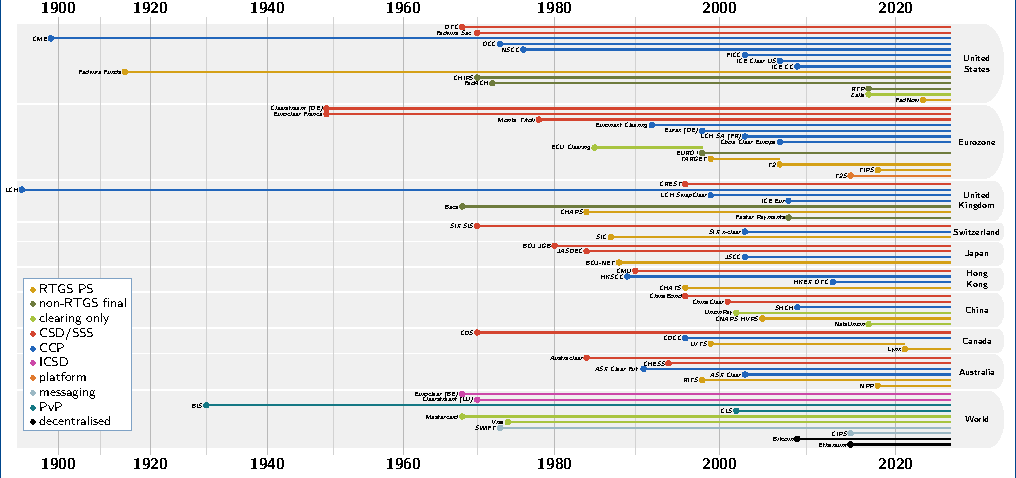
\includegraphics[width=0.96\textwidth,height=0.70\textheight,keepaspectratio]{figures/fmi-timeline-original.pdf}
  \end{center}
  \source{FMI timeline from the companion Liquidity Automata research (Kelly, UNSW).}
  \note{[Sources] Liquidity Automata FMI timeline figure. This early framing slide situates Agor\'a within a century of infrastructure consolidation before the jurisdiction tour begins.}
\end{frame}

% ============================ PART I ============================
\sectionframe{PART I}{Round the world: the eight Agor\'a jurisdictions}{the core of the briefing}

\begin{frame}{The incumbent core is already a network}
  \begin{columns}[T,onlytextwidth]
    \column{0.72\textwidth}
      \centering
      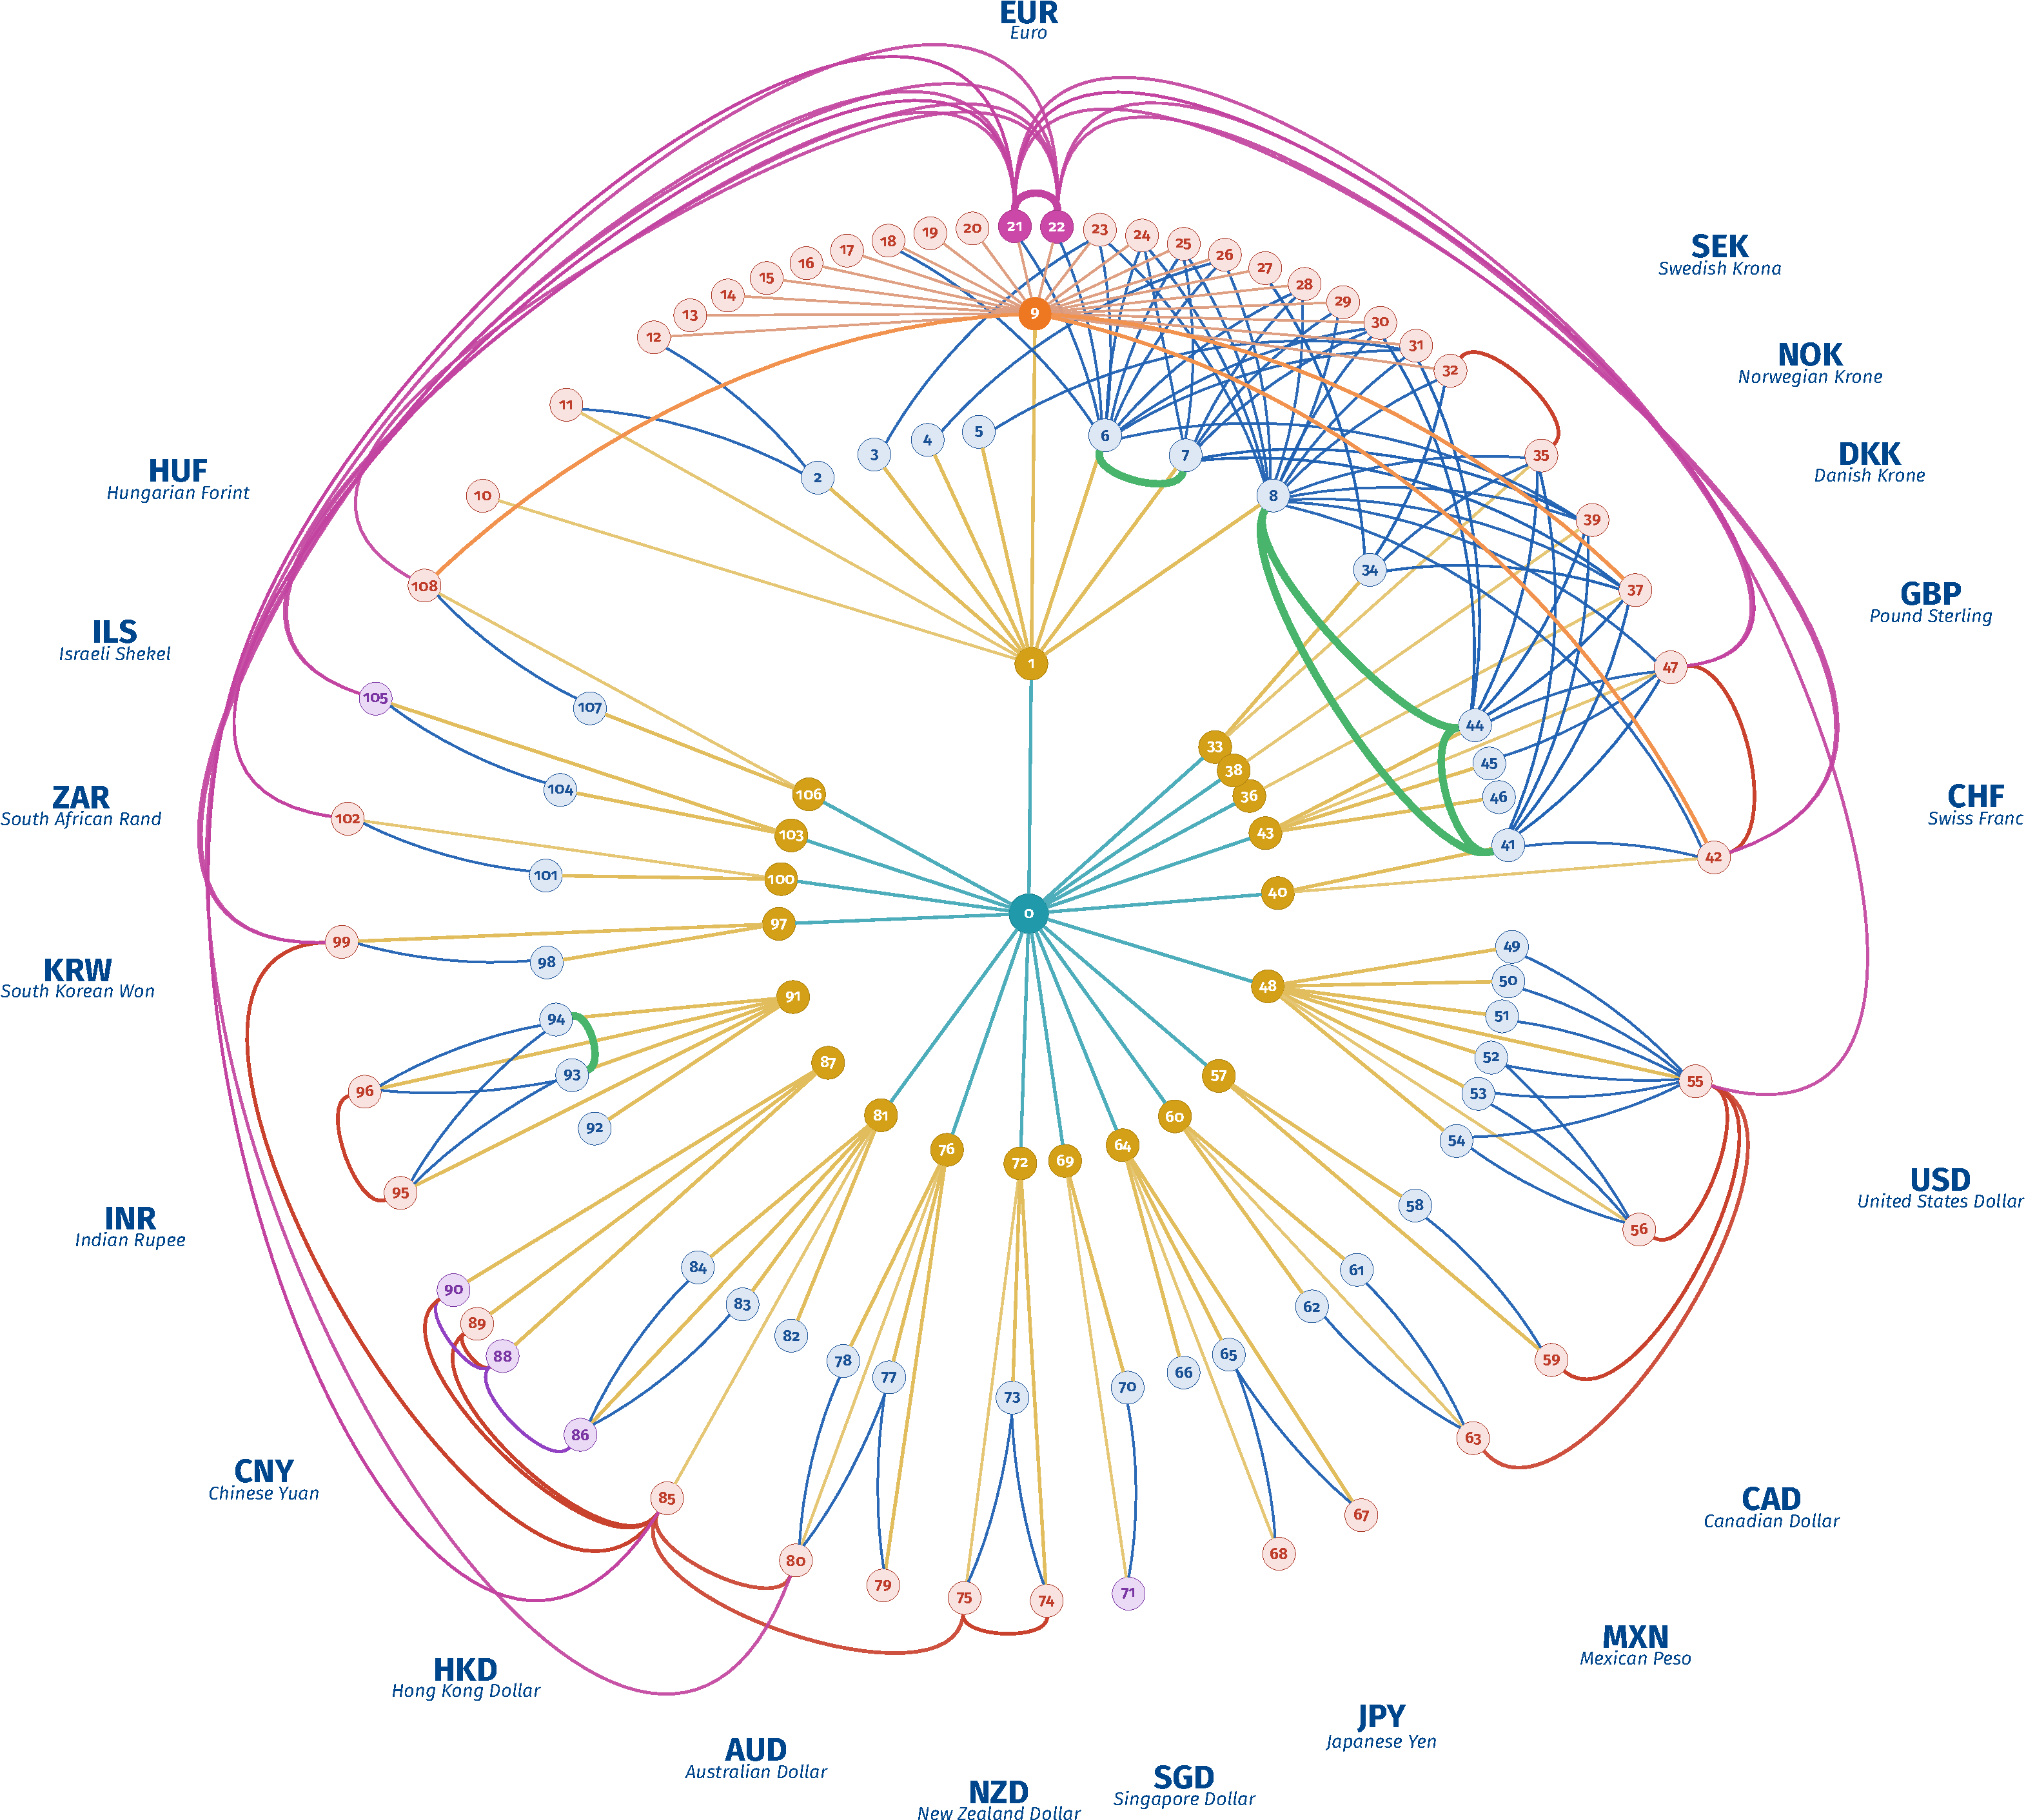
\includegraphics[width=\linewidth,height=0.72\textheight,keepaspectratio]{figures/fmi-network-networkonly-crop.pdf}
    \column{0.26\textwidth}
      \vspace{0.18cm}
      {\fontsize{7.6}{9.2}\selectfont\bfseries\color{Ocean}Node and link key\par}
      \vspace{0.10cm}
      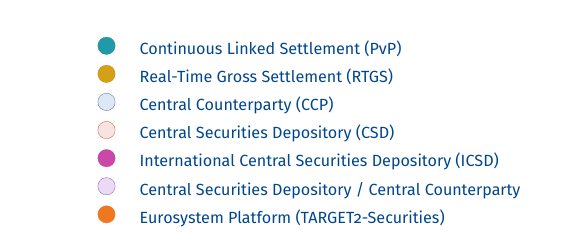
\includegraphics[width=\linewidth]{figures/fmi-network-key-nodes.png}\par
      \vspace{0.14cm}
      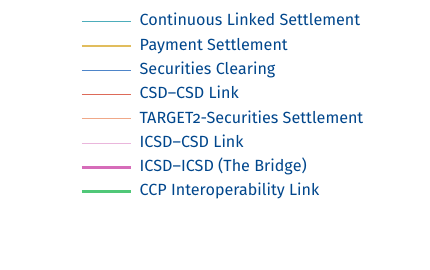
\includegraphics[width=0.80\linewidth]{figures/fmi-network-key-links.png}
  \end{columns}
  \source{Global FMI network map from the companion Liquidity Automata research (Kelly, UNSW).}
  \note{[Sources] Liquidity Automata FMI network figure: RTGS systems, CCPs, CSDs, ICSDs, T2S and CLS as nodes; membership and settlement links as edges. Framing point before the tour: every jurisdiction we visit is already embedded in this graph -- Agor\'a proposes to add a layer to it, not to draw it fresh.}
\end{frame}

\liquidityslide{figures/liquidity-automata-page-25.pdf}
\liquidityslide{figures/liquidity-automata-page-26.pdf}
\liquidityslide{figures/liquidity-automata-page-27.pdf}

% NOTE: numbers on the stack slides come from prior verified sources and the
% Liquidity Automata league tables; a verification sweep is running and any
% deltas will be patched. Japan/Korea were fully researched this session.

% --------------------------- EURO AREA ---------------------------
% ===================== REBUILT COUNTRY TOUR =====================
% --------------------------- EURO AREA ---------------------------
\begin{frame}[plain]
  \countrystrip{EUR}{eu}{Euro Area}{Payments | two public settlement services, four private schemes}
  \begin{columns}[T,onlytextwidth]
    \column{0.49\textwidth}
      \fmicard{T2}{Eurosystem}{RTGS for euro high-value payments and the cash accounts used by ancillary systems.}{Central-bank money; final on account entry; open each TARGET business day.}
      \fmicard{TIPS}{Eurosystem}{24/7 instant settlement for SCT Inst payments, reached through participant and reachable-party accounts.}{Prefunded central-bank money; transaction-by-transaction finality.}
    \column{0.49\textwidth}
      \fmicard{EURO1 / STEP2}{EBA Clearing}{Private large-value net settlement and pan-European retail batch clearing.}{EURO1 uses a single obligation structure; both settle final positions in TARGET.}
      \fmicard{RT1}{EBA Clearing}{24/7 pan-European instant-payment infrastructure for SCT Inst.}{Private scheme with prefunded settlement positions in TIPS.}
  \end{columns}
  \source{ECB TARGET Services; EBA Clearing EURO1, STEP2 and RT1 system descriptions.}
  \note{[Sources] ECB and EBA Clearing. T2 is the anchor; TIPS and private schemes solve different speed and netting problems.}
\end{frame}

\begin{frame}[plain]
  \countrystrip{EUR}{eu}{Euro Area}{Securities FMIs | settlement is shared; custody and clearing are not}
  \begin{columns}[T,onlytextwidth]
    \column{0.49\textwidth}
      \fmicard{T2S}{Eurosystem platform}{Common technical platform on which connected CSDs settle securities against dedicated cash accounts.}{DvP in central-bank money; CSDs retain their legal relationships and rulebooks.}
      \fmicard{National CSDs}{Euroclear France; Euronext Securities Milan; Iberclear}{Issue, safekeep and settle domestic securities while outsourcing the settlement engine to T2S.}{National legal records above a common Eurosystem platform.}
    \column{0.49\textwidth}
      \fmicard{ICSDs}{Euroclear Bank; Clearstream Banking Luxembourg}{Cross-border custody, settlement and collateral services, including international bonds.}{Euroclear Bank cash is commercial-bank money; Clearstream also connects to central-bank rails.}
      \fmicard{CCPs}{Eurex; LCH SA; Euronext Clearing; BME; Cboe Clear Europe}{Novate and net equity, bond, repo and derivatives exposures; collect margin and manage defaults.}{Private risk engines feeding cash and securities settlement systems.}
  \end{columns}
  \source{ECB T2S; ESMA register of authorised CSDs and CCPs; operator PFMI disclosures.}
  \note{[Sources] ECB, ESMA and operator disclosures. This reproduces the Friday deck's distinction between CSD, ICSD, CCP and settlement platform.}
\end{frame}

\begin{frame}[plain]
  \countrystrip{EUR}{eu}{Euro Area}{Digital money | retail CBDC and wholesale DLT are separate programmes}
  \begin{columns}[T,onlytextwidth]
    \column{0.49\textwidth}
      \digitalcard{Digital euro}{RETAIL CBDC}{A digital form of central-bank money for households and firms. The ECB has made no issuance decision; legislation and a later Governing Council decision remain prerequisites.}{Purpose: public money in an increasingly digital retail economy; possible first issuance from 2029 if approved.}
      \digitalcard{Pontes}{WHOLESALE BRIDGE}{Interim Eurosystem service connecting market DLT platforms to TARGET Services for settlement in central-bank money. Pilot planned from Q3 2026.}{Purpose: a central-bank cash leg for tokenised securities without replacing T2/T2S.}
    \column{0.49\textwidth}
      \digitalcard{Appia}{WHOLESALE END-STATE}{Longer-term integrated ecosystem for wholesale central-bank-money settlement of tokenised assets. A blueprint is targeted for 2028.}{Purpose: move from bilateral bridges to a common European wholesale architecture.}
      \digitalcard{Project Agor\'a}{CROSS-BORDER}{Eight euro-area banks tested tokenised deposits against tokenised reserves on a shared cross-currency workflow.}{Purpose: correspondent payment and PvP, not retail CBDC and not securities issuance.}
  \end{columns}
  \source{ECB digital euro; ECB, \href{https://www.ecb.europa.eu/press/pr/date/2026/html/ecb.pr260311~14ddf51a77.en.html}{Pontes and Appia}, 11 March 2026; BIS/IIF Agor\'a list.}
  \note{[Sources] ECB. Keep retail digital euro separate from the wholesale Pontes/Appia track.}
\end{frame}

% --------------------------- JAPAN ---------------------------
\begin{frame}[plain]
  \countrystrip{JPY}{japan}{Japan}{Payments | the central bank and Zengin split wholesale from retail}
  \begin{columns}[T,onlytextwidth]
    \column{0.49\textwidth}
      \fmicard{BOJ-NET Funds Transfer}{Bank of Japan}{RTGS for money-market, FX, securities and customer payments between account holders.}{Central-bank money; liquidity-saving features queue and offset eligible payments.}
      \fmicard{CLS yen leg}{CLS Bank with BOJ-NET}{PvP settlement of yen against other eligible currencies during the common settlement window.}{Yen funding and payouts pass through BOJ-NET accounts.}
    \column{0.49\textwidth}
      \fmicard{Zengin System}{Japanese Banks' Payment Clearing Network}{Domestic credit transfers between deposit-taking institutions; gateway for customer bank transfers.}{Multilateral net obligations settle through BOJ-NET; more-time system supports 24/7 messages.}
      \fmicard{Retail overlays}{Banks and payment providers}{Cards, QR wallets and funds-transfer services sit above bank accounts and the Zengin/BOJ-NET core.}{They change initiation and access, not the final settlement asset.}
  \end{columns}
  \source{Bank of Japan payment-system materials; Zengin-Net system description; CLS.}
  \note{[Sources] BOJ, Zengin-Net and CLS. BOJ-NET has separate funds-transfer and JGB services.}
\end{frame}

\begin{frame}[plain]
  \countrystrip{JPY}{japan}{Japan}{Securities FMIs | government bonds and private securities take different routes}
  \begin{columns}[T,onlytextwidth]
    \column{0.49\textwidth}
      \fmicard{BOJ-NET JGB Services}{Bank of Japan}{Book-entry transfer and DvP settlement for Japanese government bonds.}{Securities and cash legs settle on Bank of Japan infrastructure.}
      \fmicard{JASDEC}{Market-owned CSD}{Book-entry transfer for equities, corporate bonds, investment trusts and other private instruments.}{Links securities settlement to cash-settlement banks and BOJ-NET arrangements.}
    \column{0.49\textwidth}
      \fmicard{JSCC}{Japan Exchange Group}{CCP for cash equities, listed derivatives, OTC interest-rate swaps and government-bond transactions.}{Novation, multilateral netting, margin and default management before DvP.}
      \fmicard{Token venues}{BOOSTRY / ibet for Fin; ODX START}{Permissioned security-token registry and trading venue used for digital corporate bonds and secondary transactions.}{DCJPY supplies a programmable deposit-money cash leg; it does not clear the security itself.}
  \end{columns}
  \source{BOJ; JASDEC; JSCC; ODX and BOOSTRY system disclosures.}
  \note{[Sources] Operator materials. The last card is essential: tokenised clearing is not the same thing as the DCJPY settlement asset.}
\end{frame}

\begin{frame}[plain]
  \countrystrip{JPY}{japan}{Japan}{Digital money | CBDC research and DCJPY serve different markets}
  \begin{columns}[T,onlytextwidth]
    \column{0.49\textwidth}
      \digitalcard{BOJ CBDC pilot}{RETAIL CBDC RESEARCH}{The Bank of Japan is testing an end-to-end retail-CBDC system with intermediaries and an external expert forum. It has made no decision to issue.}{Purpose: test performance, resilience, intermediary functions and coexistence with cash and bank deposits.}
      \digitalcard{DCJPY}{TOKENISED DEPOSIT}{A bank's yen deposit liability represented on DCP's permissioned two-zone network. GMO Aozora began production issuance in August 2024.}{Financial Zone mints and burns against core deposits; Business Zones add escrow and application logic.}
    \column{0.49\textwidth}
      \digitalcard{What DCJPY settles}{ENERGY + SECURITIES}{First production use paid for digital environmental-value certificates. In 2026 escrow DvP linked DCJPY to tokenised corporate bonds and secondary-market security tokens.}{Purpose: eliminate principal risk and manual reconciliation between a token security and its bank-money cash leg.}
      \digitalcard{Project Agor\'a}{CROSS-BORDER}{Mizuho, MUFG, SBI Shinsei and SMBC tested yen deposit tokens against tokenised central-bank reserves.}{Purpose: cross-border bank payments and FX PvP; distinct from both the retail CBDC pilot and domestic securities DvP.}
  \end{columns}
  \source{BOJ, \href{https://www.boj.or.jp/en/paym/digital/index.htm}{CBDC pilot}; DCP, \href{https://www.dcjpy.com/en/pressrelease/pr-20260424.html}{security-token DvP}, 24 April 2026; BIS/IIF.}
  \note{[Sources] BOJ and DCP. DCJPY is the cash leg for tokenised securities; JSCC/JASDEC functions do not migrate into the token.}
\end{frame}

% --------------------------- KOREA ---------------------------
\begin{frame}[plain]
  \countrystrip{KRW}{south-korea}{South Korea}{Payments | a hybrid RTGS above dense retail clearing}
  \begin{columns}[T,onlytextwidth]
    \column{0.49\textwidth}
      \fmicard{BOK-Wire+}{Bank of Korea}{Hybrid high-value system combining RTGS with simultaneous bilateral and multilateral offsetting.}{Central-bank money; intraday liquidity and queuing reduce gridlock.}
      \fmicard{CLS won leg}{CLS Bank with BOK-Wire+}{PvP settlement of eligible won FX trades.}{Funding and payout connect the global FX utility to the domestic public ledger.}
    \column{0.49\textwidth}
      \fmicard{Electronic Banking System}{Korea Financial Telecommunications \& Clearings Institute}{24/7 online and mobile interbank transfers; Korea's principal retail faster-payment network.}{Transactions are immediate to users; interbank net obligations settle later in BOK-Wire+.}
      \fmicard{Other retail systems}{KFTC}{CD/ATM, giro, cheque, cash-management and local-bank networks.}{KFTC clears; the Bank of Korea settles final interbank positions.}
  \end{columns}
  \source{Bank of Korea, \href{https://www.bok.or.kr/eng/main/contents.do?menuNo=400045}{Payment and Settlement Systems}; KFTC; CLS.}
  \note{[Sources] BOK and KFTC. The instant user experience is not the same as RTGS finality between banks.}
\end{frame}

\begin{frame}[plain]
  \countrystrip{KRW}{south-korea}{South Korea}{Securities FMIs | KRX clears; KSD records and settles}
  \begin{columns}[T,onlytextwidth]
    \column{0.49\textwidth}
      \fmicard{Korea Securities Depository}{Market utility}{CSD, book-entry transfer and securities settlement for exchange and OTC markets.}{DvP cash obligations settle through designated banks or BOK-Wire+, depending on market and participant.}
      \fmicard{OTC bond settlement}{KSD + BOK-Wire+}{Institutional bond trades are matched and settled securities-against-funds.}{Central-bank-money DvP is available to eligible participants.}
    \column{0.49\textwidth}
      \fmicard{KRX cash markets}{Korea Exchange}{Exchange, market operator and CCP for listed equities and bonds.}{KRX novates and nets trades; KSD completes securities settlement.}
      \fmicard{KRX derivatives / OTC}{Korea Exchange}{CCP for listed derivatives and eligible OTC won interest-rate swaps.}{Margin and default resources sit at KRX; payments settle through banking and BOK rails.}
  \end{columns}
  \source{Bank of Korea FMI overview; KSD and KRX PFMI disclosures.}
  \note{[Sources] BOK, KSD and KRX. This slide names the operator and function instead of treating KRX and KSD as interchangeable.}
\end{frame}

\begin{frame}[plain]
  \countrystrip{KRW}{south-korea}{South Korea}{Digital money | Project Hangang rehearses a two-tier token system}
  \begin{columns}[T,onlytextwidth]
    \column{0.49\textwidth}
      \digitalcard{Wholesale CBDC}{BANK SETTLEMENT ASSET}{The Bank of Korea issues a tokenised settlement asset only to participating institutions on the shared ledger.}{Purpose: keep central-bank money at the base of tokenised bank liabilities.}
      \digitalcard{Deposit tokens}{CUSTOMER MONEY}{Participating banks issue programmable claims to customers. Phase 1 ran April to June 2025 at real merchants; Phase 2 launched in March 2026.}{Purpose: retail payment and conditional public-grant disbursement, with wallets and merchant QR acceptance.}
    \column{0.49\textwidth}
      \digitalcard{Who and how}{BOK + NINE BANKS}{BOK runs the core ledger; banks handle customer wallets, KYC and redemption. Smart-contract conditions can restrict where a grant is spent.}{Technology: shared DLT with wholesale-CBDC settlement beneath deposit tokens.}
      \digitalcard{Project Agor\'a}{CROSS-BORDER}{Hana, IBK, KB Kookmin, NongHyup, Shinhan and Woori appear in both the domestic and Agor\'a experiments.}{Agor\'a adds cross-currency path discovery and PvP; Hangang tests won use cases inside Korea.}
  \end{columns}
  \source{BOK Project Hangang Phase 1 and Phase 2 releases; BIS/IIF participant list.}
  \note{[Sources] BOK. Hangang is not a general retail CBDC: users hold bank deposit tokens; institutions settle in BOK-issued wholesale CBDC.}
\end{frame}

% --------------------------- MEXICO ---------------------------
\begin{frame}[plain]
  \countrystrip{MXN}{mexico}{Mexico}{Payments | SPEI is more than a retail transfer app}
  \begin{columns}[T,onlytextwidth]
    \column{0.49\textwidth}
      \fmicard{SPEI}{Banco de M\'exico}{Systemically important electronic transfer system for bank, government, financial-market and customer payments.}{Liquidity-saving hybrid design; final and irrevocable when settlement notices are issued.}
      \fmicard{SIAC}{Banco de M\'exico}{Master-account, liquidity and settlement service for banks and public-sector account holders.}{Provides central-bank account and liquidity functions used around other payment systems.}
    \column{0.49\textwidth}
      \fmicard{Retail access to SPEI}{Banks and non-banks}{Customer interfaces accept 24/7 transfer instructions even though the core settlement day has defined windows.}{CoDi adds QR/NFC payment requests; it moves ordinary account money and is not a CBDC.}
      \fmicard{SPID / CLS}{Banxico and CLS}{SPID handles domestic US-dollar transfers between Mexican legal entities; CLS provides PvP for eligible peso FX.}{Separate rails for domestic dollar payments and global FX settlement.}
  \end{columns}
  \source{Banco de M\'exico SPEI, SIAC, CoDi and SPID system pages; CLS.}
  \note{[Sources] Banxico and CLS. SPEI finality is tied to system notification, not the customer's app screen.}
\end{frame}

\begin{frame}[plain]
  \countrystrip{MXN}{mexico}{Mexico}{Securities FMIs | Indeval links DALI directly to central-bank cash}
  \begin{columns}[T,onlytextwidth]
    \column{0.49\textwidth}
      \fmicard{Indeval}{BMV Group CSD}{Central securities depository for government and private securities; maintains book-entry ownership records.}{Private operator under public regulation.}
      \fmicard{DALI}{Indeval}{Real-time securities settlement using DvP and optimisation of linked cash and securities instructions.}{Cash accounts are held at Banco de M\'exico; Indeval grants no settlement credit.}
    \column{0.49\textwidth}
      \fmicard{CCV}{BMV Group CCP}{Central counterparty for exchange-traded equities.}{Novates and nets obligations before DALI settlement.}
      \fmicard{Asigna}{MexDer group trust}{CCP for listed derivatives traded on MexDer.}{Collects margin, manages default exposure and settles through designated financial institutions.}
  \end{columns}
  \source{Banco de M\'exico, \href{https://www.banxico.org.mx/payment-systems/dali-securities-banco-mexico.html}{DALI}; Indeval, CCV and Asigna PFMI disclosures.}
  \note{[Sources] Banxico and operator disclosures. DALI combines a private CSD engine with cash held at the central bank.}
\end{frame}

\begin{frame}[plain]
  \countrystrip{MXN}{mexico}{Mexico}{Digital money | account-money innovation and Agor\'a}
  \begin{columns}[T,onlytextwidth]
    \column{0.49\textwidth}
      \digitalcard{CoDi}{PAYMENT OVERLAY}{QR and NFC payment requests routed through SPEI. The payer and payee still use conventional bank or e-money accounts.}{Purpose: low-cost retail acceptance and financial inclusion; it is neither tokenised money nor a digital peso.}
      \digitalcard{Retail CBDC}{NO CURRENT ISSUANCE DECISION}{Banco de M\'exico has not announced a live retail-CBDC pilot or an issuance decision. Earlier policy references do not amount to an operating system.}{This absence matters: do not relabel Agor\'a or CoDi as Mexico's retail CBDC.}
    \column{0.49\textwidth}
      \digitalcard{Project Agor\'a}{WHOLESALE CROSS-BORDER}{Banxico and BBVA M\'exico, Banorte and Monex tested tokenised reserves and bank deposits for wholesale cross-border payments.}{Purpose: pathfinding, compliance preparation and atomic multi-ledger settlement for correspondent payments and FX.}
      \digitalcard{Policy question}{ANCHOR + ACCESS}{The prototype keeps the peso settlement asset under Banxico while placing workflow and cross-border access on a shared platform.}{The unresolved issue is the production operator, rulebook and fallback if that shared layer is unavailable.}
  \end{columns}
  \source{Banco de M\'exico CoDi and payment-system disclosures; BIS Agor\'a final report; BIS/IIF participant list.}
  \note{[Sources] Banxico and BIS. The CBDC statement is deliberately limited to the absence of an announced current pilot or issuance decision.}
\end{frame}

% --------------------------- SWITZERLAND ---------------------------
\begin{frame}[plain]
  \countrystrip{CHF}{switzerland}{Switzerland}{Payments | SIX operates the rail; the SNB supplies final money}
  \begin{columns}[T,onlytextwidth]
    \column{0.49\textwidth}
      \fmicard{Swiss Interbank Clearing}{SIX Interbank Clearing under SNB mandate}{Near-continuous RTGS for high-value and retail franc payments, including instant payments.}{Final and irrevocable settlement in sight deposits at the SNB.}
      \fmicard{SIC instant payments}{SIX / SNB}{24/7 instant settlement service introduced in 2024, reached through participating banks.}{Same central-bank-money anchor, new continuous service window.}
    \column{0.49\textwidth}
      \fmicard{euroSIC}{SIX Interbank Clearing}{Swiss euro payment system linked to European payment arrangements.}{Euro settlement through the system's banking and TARGET connections, not SNB-issued money.}
      \fmicard{TWINT}{Bank-owned wallet company}{QR and app-based retail payments linked to bank accounts and cards.}{Access and messaging layer; underlying obligations ultimately settle through bank rails.}
  \end{columns}
  \source{SNB payment-system oversight; SIX SIC and euroSIC; TWINT.}
  \note{[Sources] SNB and SIX. Operating the system and issuing the settlement asset are separate institutional roles.}
\end{frame}

\begin{frame}[plain]
  \countrystrip{CHF}{switzerland}{Switzerland}{Securities FMIs | SIX spans exchange, CSD, CCP and digital venue}
  \begin{columns}[T,onlytextwidth]
    \column{0.49\textwidth}
      \fmicard{SIX SIS}{SIX Group}{Swiss CSD, custody and settlement for domestic and international securities.}{DvP through linked cash accounts and SIC arrangements.}
      \fmicard{SIX x-clear}{SIX Group}{CCP for Swiss and selected European cash-equity markets.}{Interoperates with other European CCPs; manages margin and defaults.}
    \column{0.49\textwidth}
      \fmicard{SIX Digital Exchange}{SIX Group}{Regulated exchange and CSD for natively issued digital securities.}{Production venue used by Project Helvetia for on-ledger central-bank-money DvP.}
      \fmicard{BX Digital link}{BX Swiss + SIC}{Alternative model in which tokenised securities settle while cash remains on conventional SIC accounts.}{A synchronisation mechanism joins the DLT asset leg to the public-money cash leg.}
  \end{columns}
  \source{SNB; SIX SIS, x-clear and SDX; BX Digital.}
  \note{[Sources] SNB and SIX. Switzerland deliberately operates both wCBDC-on-platform and RTGS-link models.}
\end{frame}

\begin{frame}[plain]
  \countrystrip{CHF}{switzerland}{Switzerland}{Digital money | Helvetia answers the cash-leg question directly}
  \begin{columns}[T,onlytextwidth]
    \column{0.49\textwidth}
      \digitalcard{Helvetia wCBDC}{LIVE WHOLESALE PILOT}{The SNB issues tokenised central-bank money onto SDX for eligible institutions. It has settled tokenised bonds and SNB bills in production.}{Purpose: risk-free DvP for natively digital securities; not a retail franc.}
      \digitalcard{RTGS link}{ALTERNATIVE ARCHITECTURE}{A trigger synchronises DLT securities with conventional SIC cash rather than placing wCBDC on the venue.}{Purpose: retain the existing ledger while still enabling atomic-style DvP.}
    \column{0.49\textwidth}
      \digitalcard{Who controls what}{SNB + SIX}{SNB controls issuance and redemption; SIX operates SIC, SDX and much of the securities stack.}{The public anchor remains, but operational concentration sits at the platform group.}
      \digitalcard{Project Agor\'a}{CROSS-BORDER}{UBS and Sygnum joined the bank cohort; SDX supported later testing.}{Purpose: extend the two-tier token model from Swiss securities DvP to cross-border deposits and FX settlement.}
  \end{columns}
  \source{SNB Project Helvetia releases; SIX Digital Exchange; BIS/IIF Agor\'a documentation.}
  \note{[Sources] SNB, SIX and BIS. Helvetia is wholesale central-bank money; Agor\'a also carries commercial-bank deposit claims.}
\end{frame}

% --------------------------- UNITED KINGDOM ---------------------------
\begin{frame}[plain]
  \countrystrip{GBP}{united-kingdom}{United Kingdom}{Payments | RT2 settles; schemes determine the flow}
  \begin{columns}[T,onlytextwidth]
    \column{0.49\textwidth}
      \fmicard{RT2 / CHAPS}{Bank of England}{RTGS infrastructure and high-value same-day sterling payment system.}{Direct settlement in reserves; CHAPS payments are final and irrevocable.}
      \fmicard{CREST cash link}{Bank of England + Euroclear UK \& International}{RTGS accounts provide the sterling cash leg for securities DvP in CREST.}{Central-bank money is synchronised to securities movements.}
    \column{0.49\textwidth}
      \fmicard{Faster Payments}{Pay.UK}{24/7 near-real-time retail credit transfers, including standing-order and account-to-account services.}{Scheme obligations settle on a deferred-net basis through RTGS.}
      \fmicard{Bacs}{Pay.UK}{Three-day bulk cycle for direct credits and direct debits.}{Multilateral net settlement in Bank of England money.}
  \end{columns}
  \source{Bank of England RTGS and CHAPS; Pay.UK Faster Payments and Bacs.}
  \note{[Sources] BoE and Pay.UK. RT2 is infrastructure; CHAPS, FPS and Bacs are schemes with distinct rulebooks.}
\end{frame}

\begin{frame}[plain]
  \countrystrip{GBP}{united-kingdom}{United Kingdom}{Securities FMIs | a foreign-owned CSD and three specialist CCP groups}
  \begin{columns}[T,onlytextwidth]
    \column{0.49\textwidth}
      \fmicard{CREST}{Euroclear UK \& International}{UK CSD for equities, gilts and money-market instruments; also registrar and corporate-action infrastructure.}{DvP cash settles across Bank of England accounts through the CREST/RTGS link.}
      \fmicard{LCH}{London Stock Exchange Group}{CCP for rates, repo, credit, FX and equities, including SwapClear and RepoClear.}{Global private clearing utility with margin, netting and default-management power.}
    \column{0.49\textwidth}
      \fmicard{ICE Clear Europe}{Intercontinental Exchange}{CCP for energy, credit and financial derivatives.}{Commercial settlement banks and central-bank facilities support cash flows.}
      \fmicard{LME Clear}{Hong Kong Exchanges and Clearing group}{CCP for London Metal Exchange contracts.}{Vertically integrated exchange and clearing chain for base metals.}
  \end{columns}
  \source{Bank of England recognised-payment-system and CCP pages; Euroclear, LCH, ICE and LME disclosures.}
  \note{[Sources] BoE and operators. Ownership matters because CREST, LCH and LME Clear belong to different cross-border groups.}
\end{frame}

\begin{frame}[plain]
  \countrystrip{GBP}{united-kingdom}{United Kingdom}{Digital money | four projects, four different liabilities}
  \begin{columns}[T,onlytextwidth]
    \column{0.49\textwidth}
      \digitalcard{Digital pound}{RETAIL CBDC RESEARCH}{A potential Bank of England liability for households and firms, distributed through private wallet providers. No issuance decision has been made.}{Design phase ends in 2026; Parliament and government would be involved before any launch.}
      \digitalcard{Fnality GBP}{RESERVE-BACKED SYSTEM MONEY}{Wholesale token backed by funds in an omnibus Bank of England account, used only inside Fnality's regulated payment system.}{Purpose: 24/7 programmable settlement for wholesale tokenised assets and payments.}
    \column{0.49\textwidth}
      \digitalcard{GBTD}{TOKENISED BANK DEPOSITS}{UK-bank work on interoperable digital representations of ordinary commercial-bank deposits.}{Purpose: keep bank money usable across programmable ledgers without converting every payment to stablecoin or CBDC.}
      \digitalcard{Synchronisation / wCBDC}{WHOLESALE EXPERIMENTS}{Bank of England tests link-based settlement and possible on-ledger central-bank money for DvP and cross-ledger transactions.}{Agor\'a adds the multi-currency correspondent-payment problem.}
  \end{columns}
  \source{Bank of England, \href{https://www.bankofengland.co.uk/the-digital-pound/progress-update-digital-pound-design-phase}{digital-pound progress update}; Fnality; UK Finance.}
  \note{[Sources] BoE, Fnality and UK Finance. Do not collapse a possible retail CBDC, system money and deposit tokens into one ``digital pound''.}
\end{frame}

% --------------------------- UNITED STATES ---------------------------
\begin{frame}[plain]
  \countrystrip{USD}{united-states}{United States}{Payments | competing public and bank-owned rails}
  \begin{columns}[T,onlytextwidth]
    \column{0.49\textwidth}
      \fmicard{Fedwire Funds}{Federal Reserve Banks}{RTGS for high-value and time-critical payments.}{Each transfer is final when credited in central-bank money.}
      \fmicard{FedNow / FedACH / NSS}{Federal Reserve Banks}{24/7 instant settlement, retail ACH processing and multilateral settlement for private networks.}{Three public services with different speed, credit and liquidity models.}
    \column{0.49\textwidth}
      \fmicard{CHIPS}{The Clearing House}{Large-value dollar system using prefunding, matching and offsetting to conserve liquidity.}{Bank-owned private rulebook; final positions backed by Federal Reserve account money.}
      \fmicard{RTP / EPN}{The Clearing House}{24/7 instant retail payments and private ACH processing.}{Private alternatives to FedNow and FedACH, owned by major banks.}
  \end{columns}
  \source{Federal Reserve Financial Services; The Clearing House CHIPS, RTP and EPN.}
  \note{[Sources] Federal Reserve and TCH. The United States has overlapping public and private rails rather than one national stack.}
\end{frame}

\begin{frame}[plain]
  \countrystrip{USD}{united-states}{United States}{Securities FMIs | DTCC dominates post-trade; CCPs remain specialised}
  \begin{columns}[T,onlytextwidth]
    \column{0.49\textwidth}
      \fmicard{DTC}{DTCC subsidiary}{CSD and settlement for corporate and municipal securities; receives netted obligations from NSCC.}{Net cash settles through designated commercial settlement banks.}
      \fmicard{Fedwire Securities}{Federal Reserve Banks}{Book-entry custody and transfer for Treasuries, agencies and certain international organisations.}{DvP in central-bank money over Fedwire.}
    \column{0.49\textwidth}
      \fmicard{NSCC / FICC}{DTCC subsidiaries}{CCPs for equities, government securities and mortgage-backed securities.}{Novation, netting, margin and default management before settlement.}
      \fmicard{CME / OCC / ICE}{Clearing groups and member utility}{CCPs for futures, options, rates, commodities, equities and credit.}{Specialised private risk engines above public-dollar and commercial-bank cash settlement.}
  \end{columns}
  \source{Federal Reserve; DTCC; CME Clearing; OCC; ICE Clear PFMI disclosures.}
  \note{[Sources] Federal Reserve and operator PFMI disclosures. DTC is a CSD; NSCC and FICC are CCPs.}
\end{frame}

\begin{frame}[plain]
  \countrystrip{USD}{united-states}{United States}{Digital money | private token dollars and reserve-based public money}
  \begin{columns}[T,onlytextwidth]
    \column{0.49\textwidth}
      \digitalcard{US CBDC}{NO ISSUANCE PROGRAMME}{The Federal Reserve researches digital money but has not created a retail or wholesale CBDC platform; issuance would require clear legal and political authority.}{The dollar's public digital settlement asset remains reserve balances on existing Federal Reserve systems.}
      \digitalcard{TCH deposit token}{BANK-OWNED INITIATIVE}{Shared-ledger tokenised deposits proposed by The Clearing House and member banks for round-the-clock wholesale payments and programmable settlement.}{Purpose: preserve regulated bank money while extending service beyond legacy windows.}
    \column{0.49\textwidth}
      \digitalcard{Kinexys / JPMD}{BANK DEPOSIT INFRASTRUCTURE}{JPMorgan's permissioned ledger and deposit-token services move institutional cash and support delivery-versus-payment workflows.}{Liability remains with the issuing bank; access is contractual and permissioned.}
      \digitalcard{Stablecoins + Agor\'a}{SEPARATE MODELS}{Stablecoins are non-bank or specially regulated issuer liabilities. Agor\'a instead tests tokenised bank deposits against tokenised central-bank reserves.}{US cohort: JPMorgan, Citi, BNY, FNBO and TD Bank N.A.; Visa, Mastercard and Swift also participated.}
  \end{columns}
  \source{Federal Reserve digital-currency materials; The Clearing House; Kinexys; BIS/IIF Agor\'a list.}
  \note{[Sources] Federal Reserve, TCH, JPMorgan and BIS. Programmable dollars already exist even without a US CBDC.}
\end{frame}

% --------------------------- CANADA ---------------------------
\begin{frame}[plain]
  \countrystrip{CAD}{canada}{Canada}{Payments | Lynx is live; the retail real-time rail is still arriving}
  \begin{columns}[T,onlytextwidth]
    \column{0.49\textwidth}
      \fmicard{Lynx}{Payments Canada}{Systemically important high-value payment system with RTGS and a liquidity-saving mechanism.}{Final settlement in Bank of Canada money; risk controls and collateral support intraday liquidity.}
      \fmicard{ACSS}{Payments Canada}{Batch clearing for cheques, pre-authorised debits, POS and other retail instruments.}{Multilateral net obligations settle through Lynx.}
    \column{0.49\textwidth}
      \fmicard{Interac e-Transfer}{Interac}{Near-real-time retail account-to-account service reached through participating financial institutions.}{User messaging is immediate; underlying interbank positions feed established settlement arrangements.}
      \fmicard{Real-Time Rail}{Payments Canada + Interac}{ISO 20022 instant-payment system intended to add 24/7 irrevocable retail payments and richer data.}{Target launch Q4 2026; designed to settle in central-bank money.}
  \end{columns}
  \source{Payments Canada Lynx, ACSS and Real-Time Rail; Interac.}
  \note{[Sources] Payments Canada and Interac. Do not describe Interac e-Transfer as the missing RTR: they have different settlement and access designs.}
\end{frame}

\begin{frame}[plain]
  \countrystrip{CAD}{canada}{Canada}{Securities FMIs | TMX owns both the depository and domestic CCP}
  \begin{columns}[T,onlytextwidth]
    \column{0.49\textwidth}
      \fmicard{CDS / CDSX}{TMX Group}{Canadian CSD, clearing and settlement infrastructure for equities, debt and money-market instruments.}{Securities move in CDSX; payment obligations settle through designated banks and Bank of Canada arrangements.}
      \fmicard{CDCC}{TMX Group}{CCP for listed derivatives, fixed-income transactions and selected equity products.}{Margin, netting and default management are vertically integrated with the exchange group.}
    \column{0.49\textwidth}
      \fmicard{CCMS}{TMX + Clearstream}{Collateral inventory, mobilisation and optimisation service linking Canadian market participants.}{It changes collateral selection and movement; it is not a payment system or digital Canadian dollar.}
      \fmicard{Public oversight}{Bank of Canada + provincial regulators}{The Bank designates and oversees systemically important systems; securities regulation remains provincial.}{Ownership, operation, supervision and settlement asset are separate control layers.}
  \end{columns}
  \source{Bank of Canada designated FMIs; TMX CDS, CDCC and CCMS disclosures.}
  \note{[Sources] BoC and TMX. CCMS is included because it optimises collateral across the FMI stack, not because it issues money.}
\end{frame}

\begin{frame}[plain]
  \countrystrip{CAD}{canada}{Canada}{Digital money | contingency research, then Agor\'a accession}
  \begin{columns}[T,onlytextwidth]
    \column{0.49\textwidth}
      \digitalcard{Retail CBDC}{CONTINGENCY RESEARCH}{The Bank of Canada completed extensive design research and moved active development into a readiness programme; issuance would depend on future need and public authority.}{Purpose: preserve the capacity to respond if cash use collapses or private digital money threatens monetary sovereignty.}
      \digitalcard{Project Jasper}{WHOLESALE PRECURSOR}{Earlier Bank of Canada experiments tested DLT wholesale payments, securities DvP and cross-border settlement.}{Purpose: understand whether distributed systems improve existing institutional markets.}
    \column{0.49\textwidth}
      \digitalcard{Project Agor\'a}{JOINED MAY 2026}{Canada joined after the seven-currency prototype report, bringing the Bank of Canada and a new Canadian private-sector cohort into later exploration.}{Purpose: test the two-tier cross-border model against Canada's Lynx-centred monetary architecture.}
      \digitalcard{CCMS}{COLLATERAL INFRASTRUCTURE}{The live TMX/Clearstream service mobilises and optimises securities collateral; the Bank of Canada plans to use it for market operations.}{Purpose: coordinate production collateral inventory and movement across participating institutions.}
  \end{columns}
  \source{Bank of Canada digital-dollar and Jasper materials; BIS, 27 May 2026; TMX/Clearstream CCMS.}
  \note{[Sources] BoC, BIS and TMX. Canada was not one of the seven original prototype currencies.}
\end{frame}

% --------------------------- COMPARISON ---------------------------
\begin{frame}[shrink=20]{Eight stacks, one comparison}
  \fontsize{7.6}{9.15}\selectfont
  \begin{tabularx}{\textwidth}{L{1.05cm}L{1.35cm}L{2.65cm}L{2.4cm}Y}
    \toprule
    \textbf{Area} & \textbf{Public cash anchor} & \textbf{Core securities FMIs} & \textbf{Digital-money path} & \textbf{What is actually being settled} \\
    \midrule
    Euro & T2 / TIPS & T2S; Euroclear; Clearstream; CCPs & digital euro; Pontes; Appia & retail public money vs token-security cash leg \\
    Japan & BOJ-NET & BOJ JGB; JASDEC; JSCC & BOJ CBDC pilot; DCJPY & retail CBDC research vs deposit-token DvP \\
    Korea & BOK-Wire+ & KSD; KRX CCP & Hangang; Agor\'a & deposit tokens over wholesale CBDC \\
    Mexico & SPEI / SIAC & Indeval DALI; CCV; Asigna & CoDi; Agor\'a & account money vs cross-border token claims \\
    Switzerland & SIC & SIX SIS; x-clear; SDX & Helvetia; RTGS link & tokenised bonds against wCBDC or SIC cash \\
    UK & RT2 & CREST; LCH; ICE; LME & digital pound; Fnality; GBTD & retail CBDC research, system money, deposits \\
    US & Fedwire / FedNow & DTC; NSCC/FICC; CME/OCC/ICE & TCH; Kinexys; stablecoins & private token dollars, no Fed CBDC token \\
    Canada & Lynx & CDS; CDCC; CCMS & CBDC contingency; Agor\'a & wholesale claims; collateral optimisation \\
    \bottomrule
  \end{tabularx}
  \source{Central-bank and FMI sources listed on the preceding 24 jurisdiction slides.}
  \note{[Sources] Preceding slides. The last column prevents four legally different instruments from being called ``CBDC''.}
\end{frame}

% ============================ PART II ============================
\sectionframe{PART II}{Project Agora Principles}{what was built, what was found, what remains open}
% ===================== REBUILT AGORA REPORT WALKTHROUGH =====================
\begin{frame}[shrink=20]{Seven questions organise the findings}
  \reporttag{REPORT STRUCTURE}\par\vspace{0.10cm}
  \fontsize{8.3}{10}\selectfont
  \begin{tabularx}{\textwidth}{L{3.55cm}Y}
    \toprule
    \textbf{Question answered} & \textbf{What the report contributes} \\
    \midrule
    Why Agor\'a? & vision, participants, objectives and explicit assumptions \\
    What must improve? & pain points, 15 business requirements and design choices \\
    What was built? & prototype architecture and end-to-end / PvP workflows \\
    How did it work? & ledger, contracts, participant suite, privacy and testing \\
    Could it be legal? & asset character, finality, compliance, data and rulebooks \\
    Did it help? & three scenarios, qualitative benefits and limitations \\
    What comes next? & outcomes and technical, functional and legal work \\
    \bottomrule
  \end{tabularx}
  \vspace{0.12cm}
  \begin{statement}
    The report establishes prototype feasibility; production still requires an operator, rulebook, resilience regime and launch decision.
  \end{statement}
  \source{BIS, \href{https://www.bis.org/publ/othp110.pdf}{Project Agor\'a final report}, 27 May 2026, contents and Executive Summary.}
  \note{[Sources] BIS final report, 97 pages. This frame is the navigation for the next sequence.}
\end{frame}

\begin{frame}{42 private participants: global and European banks}
  \fontsize{9.7}{11.5}\selectfont
  \begin{columns}[T,onlytextwidth]
    \column{0.32\textwidth}
      \begin{itemize}\verytightitems
        \item BNP Paribas
        \item BNY
        \item Citi
        \item Cr\'edit Agricole CIB
        \item Deutsche Bank
        \item HSBC
      \end{itemize}
    \column{0.32\textwidth}
      \begin{itemize}\verytightitems
        \item JPMorgan Chase
        \item Standard Chartered
        \item UBS
        \item Santander
        \item BBVA
        \item CaixaBank
      \end{itemize}
    \column{0.32\textwidth}
      \begin{itemize}\verytightitems
        \item Commerzbank
        \item Groupe BPCE
        \item Lloyds Banking Group
        \item NatWest Group
        \item FNBO
        \item TD Bank N.A.
      \end{itemize}
  \end{columns}
  \begin{statement}
    Eighteen of the 42 private participants are global, European or US banks; the cohort spans issuers, correspondents and potential liquidity providers.
  \end{statement}
  \source{BIS, Project Agor\'a report, participant roster, May 2026.}
  \note{[Sources] BIS Project Agor\'a report, inside-cover participant roster. TD Bank N.A. is the US subsidiary; Canada joined the public-sector project after this roster was fixed.}
\end{frame}

\begin{frame}[shrink=12]{42 private participants: regional banks}
  \fontsize{8.9}{10.7}\selectfont
  \begin{columns}[T,onlytextwidth]
    \column{0.24\textwidth}
      \rust{Japan}
      \begin{itemize}\verytightitems
        \item Mizuho Bank
        \item MUFG Bank
        \item SBI Shinsei Bank
        \item SMBC
      \end{itemize}
    \column{0.24\textwidth}
      \blue{South Korea}
      \begin{itemize}\verytightitems
        \item Hana Bank
        \item IBK
        \item KB Kookmin Bank
        \item NongHyup Bank
        \item Shinhan Bank
        \item Woori Bank
      \end{itemize}
    \column{0.24\textwidth}
      \rust{Switzerland}
      \begin{itemize}\verytightitems
        \item AMINA Bank
        \item Banque Cantonale Vaudoise
        \item Basler Kantonalbank
        \item PostFinance
        \item Sygnum Bank
      \end{itemize}
    \column{0.24\textwidth}
      \blue{Latin America}
      \begin{itemize}\verytightitems
        \item Banco BV
        \item Banorte
        \item Monex
      \end{itemize}
  \end{columns}
  \vspace{0.08cm}
  {\fontsize{8.8}{10.5}\selectfont\bfseries Eighteen regional banks supply domestic account, compliance and currency expertise.\par}
  \source{BIS, Project Agor\'a report, participant roster, May 2026.}
  \note{[Sources] BIS final-report roster. Regional headings describe head-office geography, not the full legal footprint of each group.}
\end{frame}

\begin{frame}[shrink=12]{42 private participants: FMIs and networks}
  \fontsize{9.6}{11.5}\selectfont
  \begin{tabularx}{\textwidth}{L{3.0cm}Y}
    \toprule
    \textbf{Participant} & \textbf{Capability represented in the cohort} \\
    \midrule
    Eurex Clearing & CCP risk management, margin, default management and settlement dependencies \\
    Euroclear & CSD/ICSD settlement, custody, collateral and cross-border securities links \\
    SIX Digital Exchange & regulated DLT exchange and CSD operations \\
    Mastercard & network rules, identity, risk controls and bank distribution \\
    Visa & network rules, risk controls and tokenised-bank-liability initiatives \\
    Swift & ISO 20022 connectivity, identity and a competing shared-ledger programme \\
    \bottomrule
  \end{tabularx}
  \vspace{0.08cm}
  {\fontsize{8.8}{10.5}\selectfont\bfseries Six infrastructure participants contribute clearing, custody, securities settlement, network and messaging capabilities.\par}
  \source{BIS, Project Agor\'a report, participant roster, May 2026; participant disclosures.}
  \note{[Sources] BIS final-report roster and operator descriptions. 36 banks plus these six organisations equals 42 private participants.}
\end{frame}

\begin{frame}[shrink=30]{The correspondent workflow}
  \reporttag{WHY CHANGE THE WORKFLOW}\par\vspace{0.12cm}
  \begin{columns}[T,onlytextwidth]
    \column{0.47\textwidth}
      \rust{Why the current chain is costly}
      \begin{itemize}\verytightitems
        \item Multiple ledgers update sequentially.
        \item Compliance and data checks repeat at each hop.
        \item Operating hours and cut-offs do not align.
        \item Liquidity is prefunded across correspondent accounts.
        \item Exceptions trigger bilateral investigation and reconciliation.
      \end{itemize}
    \column{0.49\textwidth}
      \blue{The unified-ledger proposition}
      \begin{itemize}\verytightitems
        \item Put tokenised commercial-bank deposits and central-bank reserves into one coordinated workflow.
        \item Preserve two-tier banking and the singleness of money.
        \item Prepare payment legs and compliance in parallel.
        \item Commit the complete transaction, or cancel it.
      \end{itemize}
  \end{columns}
  \source{BIS Agor\'a final report, Executive Summary and Chapter 1.}
  \note{[Sources] Report pp. 1--15. The 2024 cross-border market estimate is omitted here so the architecture, not market sizing, leads.}
\end{frame}

\begin{frame}[shrink=30]{Four objectives and hard boundaries}
  \reporttag{OBJECTIVES + BOUNDARIES}\par\vspace{0.10cm}
  \begin{columns}[T,onlytextwidth]
    \column{0.47\textwidth}
      \rust{Four objectives}
      \begin{enumerate}\verytightitems
        \item \textbf{Interoperability} across money and currency ledgers.
        \item \textbf{Programmability and composability} of the workflow.
        \item \textbf{Atomic settlement} across every required payment leg.
        \item \textbf{Enhanced compliance} using richer, reusable outcomes.
      \end{enumerate}
    \column{0.49\textwidth}
      \blue{What the prototype assumed}
      \begin{itemize}\verytightitems
        \item Each central bank retains account and access policy.
        \item Banks can fund tokens from existing systems.
        \item The platform is the golden source for token balances.
        \item Production scalability, cyber resilience, liquidity-saving, live FX and tokenised securities are out of scope.
      \end{itemize}
  \end{columns}
  \begin{statement}
    Agor\'a established prototype feasibility. Systemic operation still requires live integration, resilience and market-scale evidence.
  \end{statement}
  \source{BIS Agor\'a final report, Chapter 1.}
  \note{[Sources] Chapter 1 objectives and assumptions. Seven central banks and 40 private institutions contributed to the reported prototype; Canada joined later exploration.}
\end{frame}

\begin{frame}[shrink=35]{Fifteen business requirements}
  \reporttag{BUSINESS REQUIREMENTS}\par\vspace{0.08cm}
  \fontsize{7.8}{9.45}\selectfont
  \begin{columns}[T,onlytextwidth]
    \column{0.49\textwidth}
      \fmicard{Authority and money}{R1--R3}{Preserve issuer autonomy; support issuance, redemption and transfer; manage settlement risk atomically.}{A shared workflow must not erase central-bank or commercial-bank control of its own liability.}
      \fmicard{Route and integrity}{R4--R5}{Find viable correspondent paths and preserve cross-currency integrity across all legs.}{No partial value transfer when one currency leg fails.}
      \fmicard{Access and compliance}{R6--R7}{Authorise only permitted actors; prevalidate sanctions, AML/KYC, fraud and payment data.}{Checks remain institution-specific even when outcomes are shared.}
      \fmicard{Standards and exceptions}{R8--R9}{Use ISO 20022 / CBPR+ / HVPS+; support investigation, repair, return and cancellation.}{The happy path is not enough for production payments.}
    \column{0.49\textwidth}
      \fmicard{Visibility and privacy}{R10--R11}{Give participants useful status and reporting while selectively sharing transaction data.}{Common state need not mean universal data access.}
      \fmicard{Liquidity and governance}{R12--R13}{Monitor liquidity and define operational, issuer and participant roles.}{The prototype tests balances; production needs institutions.}
      \fmicard{Non-functional controls}{R14}{Reliability, security, scalability, performance and recoverability.}{Required by the business specification but not performance-tested.}
      \fmicard{Finality}{R15}{Make completion legally and operationally irreversible in every affected jurisdiction.}{Technical commit and legal finality must be aligned, not assumed.}
  \end{columns}
  \source{BIS Agor\'a final report, Chapter 2, requirements 1--15.}
  \note{[Sources] Chapter 2. Requirements are grouped without changing their order or substance.}
\end{frame}

\begin{frame}[shrink=30]{Five design choices}
  \reporttag{DESIGN PRINCIPLES}\par\vspace{0.12cm}
  \begin{enumerate}\tightitems
    \item \rust{Coordinate balance updates} across central-bank and commercial-bank ledgers instead of moving every claim onto one ledger.
    \item \rust{Confirm the payee} before value moves, reducing misdirection and unusable beneficiary data.
    \item \rust{Discover a path} through correspondents before instructing the full chain.
    \item \rust{Share compliance outcomes, not complete case files}; each institution keeps its own controls and evidential record.
    \item \rust{Lock first, then commit atomically}: each money issuer reserves its leg and delegates only the limited authority needed for settlement.
  \end{enumerate}
  \vspace{0.10cm}
  \begin{statement}
    The innovation is coordination: information and liquidity are prepared in parallel, then a single workflow decides commit or cancel.
  \end{statement}
  \source{BIS Agor\'a final report, Chapter 2.}
  \note{[Sources] Chapter 2 business challenges, requirements and design decisions.}
\end{frame}

\begin{frame}[shrink=25]{Two ledger layers preserve two-tier money}
  \reporttag{TWO-LAYER ARCHITECTURE}\par\vspace{0.08cm}
  \begin{center}
  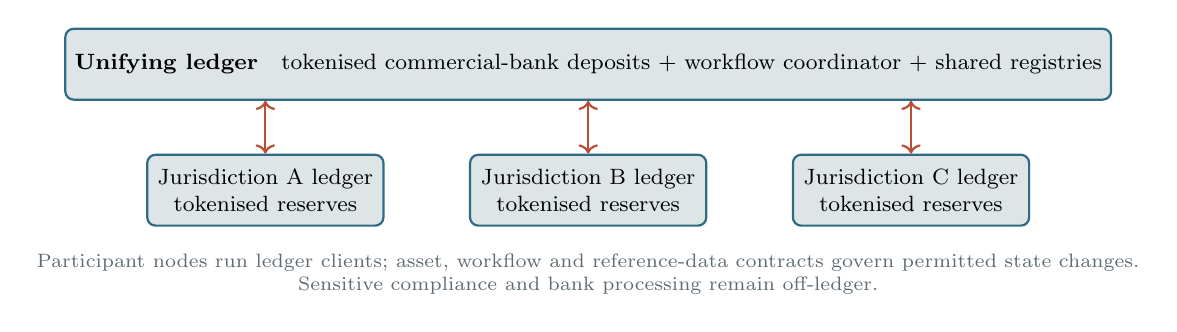
\begin{tikzpicture}[
    box/.style={draw=Ocean,thick,rounded corners=3pt,fill=Mist,minimum height=.9cm,align=center,font=\fontsize{8}{9.5}\selectfont},
    arr/.style={-{Latex[length=5pt]},thick,draw=Rust}
  ]
    \node[box,minimum width=11.4cm] (u) at (0,1.55) {\textbf{Unifying ledger}\quad tokenised commercial-bank deposits + workflow coordinator + shared registries};
    \node[box,minimum width=3.0cm] (j1) at (-4.1,-.05) {Jurisdiction A ledger\\tokenised reserves};
    \node[box,minimum width=3.0cm] (j2) at (0,-.05) {Jurisdiction B ledger\\tokenised reserves};
    \node[box,minimum width=3.0cm] (j3) at (4.1,-.05) {Jurisdiction C ledger\\tokenised reserves};
    \draw[arr,<->] (u.south -| j1.north) -- (j1.north);
    \draw[arr,<->] (u.south -| j2.north) -- (j2.north);
    \draw[arr,<->] (u.south -| j3.north) -- (j3.north);
    \node[font=\fontsize{7}{8.4}\selectfont,text=Quiet,align=center] at (0,-1.12) {Participant nodes run ledger clients; asset, workflow and reference-data contracts govern permitted state changes.\\Sensitive compliance and bank processing remain off-ledger.};
  \end{tikzpicture}
  \end{center}
  \begin{statement}
    The unified workflow preserves separate balance sheets: deposits remain claims on named banks and reserve tokens remain claims on named central banks.
  \end{statement}
  \source{BIS Agor\'a final report, Chapter 3.}
  \note{[Sources] Chapter 3 architecture. The diagram simplifies the prototype's unifying and jurisdiction-specific ledgers.}
\end{frame}

\begin{frame}[shrink=35]{The five-stage payment workflow}
  \reporttag{PAYMENT WORKFLOW}\par\vspace{0.06cm}
  \fontsize{8.2}{9.8}\selectfont
  \begin{enumerate}\tightitems
    \item \rust{Confirmation of payee}: payer and payee banks compare names and account data inside a temporary privacy group; the workflow retains the match outcome.
    \item \rust{Payment discovery and matching}: banks exchange bilateral capacity and conditions hop by hop; the search can backtrack until it finds an executable correspondent path.
    \item \rust{Validation}: every bank performs sanctions, AML/KYC, fraud, amount and operational-readiness checks, reporting only prescribed outcomes.
    \item \rust{Lock and delegate}: each issuer locks the required deposit or reserve balance and gives a smart contract narrowly scoped, temporary spending authority.
    \item \rust{Settle or cancel}: the coordinator verifies all locks, spends every leg, and completes the workflow; if prerequisites fail, locks are cancelled.
  \end{enumerate}
  \begin{statement}
    Agor\'a's atomicity is a workflow guarantee across ledgers. Legal finality requires a separate rulebook and statutory analysis.
  \end{statement}
  \source{BIS Agor\'a final report, Chapter 3.}
  \note{[Sources] Chapter 3. CoP means confirmation of payee; PDM means payment discovery and matching.}
\end{frame}

\begin{frame}[shrink=30]{The technical stack}
  \reporttag{TECHNICAL STACK}\par\vspace{0.10cm}
  \begin{columns}[T,onlytextwidth]
    \column{0.48\textwidth}
      \rust{Ledger and consensus}
      \begin{itemize}\verytightitems
        \item Hyperledger Besu, Ethereum Virtual Machine compatible.
        \item Permissioned validators using QBFT proof of authority.
        \item Deterministic contract execution and ledger ordering.
      \end{itemize}
      \rust{Asset functions}
      \begin{itemize}\verytightitems
        \item Mint, burn and transfer.
        \item Create, delegate, spend and cancel a lock.
      \end{itemize}
    \column{0.48\textwidth}
      \blue{Workflow and reference contracts}
      \begin{itemize}\verytightitems
        \item Coordinator on the unifying ledger.
        \item Payment-leg contracts on each relevant ledger.
        \item Network, token, corridor and reserve-account registries.
      \end{itemize}
      \blue{Important qualification}
      \begin{itemize}\verytightitems
        \item QBFT gives deterministic technical state.
        \item It does not by itself create legal settlement finality.
      \end{itemize}
  \end{columns}
  \source{BIS Agor\'a final report, Chapter 4.}
  \note{[Sources] Chapter 4 ledger architecture and contract specifications.}
\end{frame}

\begin{frame}[shrink=25]{The participant suite}
  \reporttag{PARTICIPANT SUITE}\par\vspace{0.08cm}
  \begin{center}
  
\begin{tikzpicture}[
    unit/.style={draw=Ocean!80,thick,rounded corners=3pt,fill=Mist,minimum width=2.15cm,minimum height=.88cm,align=center,font=\fontsize{7.2}{8.5}\selectfont},
    arr/.style={-{Latex[length=4.5pt]},thick,draw=Rust}
  ]
    \node[unit] (ui) at (-5.2,0) {User interface\\operations};
    \node[unit] (api) at (-2.6,0) {OpenAPI\\ISO 20022 edge};
    \node[unit] (mid) at (0,0) {Middleware\\bank controls};
    \node[unit] (node) at (2.6,0) {Ledger node\\smart contracts};
    \node[unit] (idx) at (5.2,0) {Indexer\\reporting};
    \draw[arr] (ui) -- (api); \draw[arr] (api) -- (mid); \draw[arr] (mid) -- (node); \draw[arr] (node) -- (idx);
    \node[font=\fontsize{7.2}{8.5}\selectfont,text=Quiet,align=center] at (0,-1.15) {pacs.008 and pacs.009 messages enter at the edge; middleware performs bank-specific checks and translates them into permitted ledger actions.};
  \end{tikzpicture}
  \end{center}
  \begin{itemize}\verytightitems
    \item Institutions can deploy components across cloud, multiple clouds or on-premises environments.
    \item Sensitive screening logic and case evidence stay within the bank's control boundary.
    \item The report leaves the production operator and hosting/governance model undecided.
  \end{itemize}
  \source{BIS Agor\'a final report, Chapter 4.}
  \note{[Sources] Chapter 4 participant suite, APIs, ISO 20022 and deployment.}
\end{frame}

\begin{frame}[shrink=35]{Privacy, PvP and assurance}
  \reporttag{PRIVACY + PVP + ASSURANCE}\par\vspace{0.08cm}
  \begin{columns}[T,onlytextwidth]
    \column{0.48\textwidth}
      \rust{Selective visibility}
      \begin{itemize}\verytightitems
        \item Privacy groups isolate bilateral or limited-party processing.
        \item Confirmation-of-payee data can be processed ephemerally.
        \item The shared ledger stores only the state and outcomes required to advance the workflow.
      \end{itemize}
      \rust{PvP special case}
      \begin{itemize}\verytightitems
        \item No payee confirmation, path search or customer amount is needed.
        \item Both currency legs validate and lock; the coordinator commits or cancels both.
      \end{itemize}
    \column{0.48\textwidth}
      \blue{What testing established}
      \begin{itemize}\verytightitems
        \item Four milestone cycles and participant user-acceptance testing.
        \item Functional execution of selected scenarios.
        \item Qualitative assessment of the business requirements.
      \end{itemize}
      \blue{What it did not establish}
      \begin{itemize}\verytightitems
        \item No stress, throughput or latency benchmark.
        \item No production cyber, failover or resilience test.
        \item No live RTGS or core-banking integration.
      \end{itemize}
  \end{columns}
  \source{BIS Agor\'a final report, Chapter 4.}
  \note{[Sources] Chapter 4 privacy, PvP and UAT sections.}
\end{frame}

\begin{frame}[shrink=35]{What the tokens are in law}
  \reporttag{LEGAL CHARACTER OF MONEY}\par\vspace{0.08cm}
  \fontsize{9.2}{11}\selectfont
  \begin{itemize}\tightitems
    \item A reserve token is the definitive platform record of an underlying central-bank reserve-account balance; a deposit token records a named bank's deposit liability.
    \item The legal debtor-creditor relationship remains with the issuer. The token records that existing claim against a named bank or central bank.
    \item Minting and burning correspond to credits and debits of the relevant account; transfer changes the recorded account balance.
    \item Smart-contract code executes rights and duties established by the governing law, rulebook and participant agreements.
    \item Eligible direct actors are central banks and commercial banks; an FMI or CCP may initiate a PvP workflow. NBFIs and corporates participate indirectly through banks; natural persons are outside scope.
  \end{itemize}
  \begin{statement}
    The prototype preserves familiar money law, but only if contracts and public law make the ledger entry authoritative.
  \end{statement}
  \source{BIS Agor\'a final report, Chapter 5.}
  \note{[Sources] Chapter 5 roles and legal nature of reserves and deposits.}
\end{frame}

\begin{frame}[shrink=30]{The legal finality trigger}
  \reporttag{FINALITY}\par\vspace{0.08cm}
  \begin{enumerate}\tightitems
    \item Each issuer first locks its own balance and delegates only the authority needed for the transaction.
    \item Because the ledgers update asynchronously, the report identifies an \rust{atomic settlement trigger} on the unifying ledger.
    \item The production rulebook would need that trigger to mark irrevocability, finality and discharge in every participating jurisdiction.
    \item Insolvency law and any payment-system designation must recognise that result; otherwise a technically complete transfer may remain legally contestable.
    \item Choice of law, mandatory local law and public policy may still produce jurisdiction-specific differences.
  \end{enumerate}
  \begin{statement}
    Atomic execution is a software fact. Finality is a legal allocation of when nobody may unwind the payment.
  \end{statement}
  \source{BIS Agor\'a final report, Chapter 5, finality and choice-of-law analysis.}
  \note{[Sources] Chapter 5. This is the report's most important bridge between the prototype and a production system.}
\end{frame}

\begin{frame}[shrink=35]{Compliance and data}
  \reporttag{COMPLIANCE + DATA}\par\vspace{0.08cm}
  \begin{columns}[T,onlytextwidth]
    \column{0.48\textwidth}
      \rust{Financial-crime controls}
      \begin{itemize}\verytightitems
        \item Every bank performs its own sanctions, AML/KYC and fraud checks.
        \item Three prescribed pass/fail outcomes govern whether the workflow advances.
        \item Failure flags can create confidentiality or tipping-off risks.
        \item Regulators may need evidence beyond a binary outcome.
      \end{itemize}
    \column{0.48\textwidth}
      \blue{Privacy and localisation}
      \begin{itemize}\verytightitems
        \item Privacy groups reduce disclosure but do not eliminate personal data.
        \item Customer consent may be needed for payee checks and outcome sharing.
        \item Korea imposes strict localisation constraints; Mexico requires some domestic logs and accounting records.
        \item Supervisory access and cross-border transfer rules differ by jurisdiction.
      \end{itemize}
  \end{columns}
  \begin{statement}
    Shared outcomes reduce repetition only if secrecy, evidential and localisation rules let institutions rely on them.
  \end{statement}
  \source{BIS Agor\'a final report, Chapter 5.}
  \note{[Sources] Chapter 5 financial-crime, privacy and data-localisation sections.}
\end{frame}

\begin{frame}[shrink=30]{Three benefit scenarios}
  \reporttag{BENEFITS}\par\vspace{0.08cm}
  \fontsize{8.25}{9.9}\selectfont
  \begin{tabularx}{\textwidth}{L{2.15cm}L{2.35cm}Y Y}
    \toprule
    \textbf{Scenario} & \textbf{Problem} & \textbf{Agor\'a mechanism} & \textbf{Claimed benefit} \\
    \midrule
    Mexico to US urgent invoice & known correspondent path; time-sensitive US\$200k payment & parallel validation and liquidity locks across deposit and reserve tokens & shorter workflow, less reconciliation and lower settlement exposure \\
    Switzerland to Korea corporate payment & route initially unknown; EUR used as vehicle currency & confirmation of payee, path discovery, validation and coordinated settlement & better route visibility and reduced manual outreach \\
    UK to Japan liquidity rebalance & two correspondents exchange GBP and JPY & validate, lock both currency legs and execute PvP & removal of principal risk from asynchronous FX settlement \\
    \bottomrule
  \end{tabularx}
  \vspace{0.10cm}
  \begin{statement}
    The chapter identifies plausible sources of value; production cost, realised savings and market-wide liquidity effects remain unquantified.
  \end{statement}
  \source{BIS Agor\'a final report, Chapter 6.}
  \note{[Sources] Chapter 6 real-life scenarios and benefits assessment.}
\end{frame}

\begin{frame}[shrink=30]{The prototype's limits}
  \reporttag{PROTOTYPE LIMITATIONS}\par\vspace{0.08cm}
  \begin{columns}[T,onlytextwidth]
    \column{0.48\textwidth}
      \rust{Not production-tested}
      \begin{itemize}\verytightitems
        \item Cybersecurity and adversarial resilience
        \item Throughput, latency and peak-volume stress
        \item Node, network and regional failover
        \item Operational monitoring and incident response
        \item RTGS, core-banking and live compliance integration
      \end{itemize}
    \column{0.48\textwidth}
      \blue{Not fully solved}
      \begin{itemize}\verytightitems
        \item Liquidity-saving and queue management
        \item Fee transparency to end customers
        \item Exception handling and customer outreach
        \item Production governance and operator model
        \item Cross-jurisdiction legal finality and insolvency
      \end{itemize}
  \end{columns}
  \begin{statement}
    A successful prototype can still leave the expensive parts of a systemic utility almost entirely ahead.
  \end{statement}
  \source{BIS Agor\'a final report, Chapter 6.}
  \note{[Sources] Chapter 6 limitations. This slide is not criticism external to the report; these caveats are the report's own.}
\end{frame}

\begin{frame}[shrink=30]{Six outcomes}
  \reporttag{OUTCOMES}\par\vspace{0.08cm}
  \begin{enumerate}\tightitems
    \item Tokenisation can improve the \rust{workflow around money}, not only represent balances differently.
    \item Public-private collaboration is necessary because central banks issue the anchor while commercial banks own customer and compliance processes.
    \item A shared ledger can preserve issuer autonomy through separate assets, permissions and jurisdictional domains.
    \item Tokenisation does not inherently change the legal nature of reserves or deposits.
    \item Shared infrastructure does not require every participant to see every data item.
    \item Interoperability among bank deposit tokens is central to preserving singleness in a multi-bank system.
  \end{enumerate}
  \begin{statement}
    The result is a defensible two-tier architecture. Selection of a market utility requires a separate institutional decision.
  \end{statement}
  \source{BIS Agor\'a final report, Chapter 7.}
  \note{[Sources] Chapter 7 outcomes. The final sentence is the briefing's inference from those findings.}
\end{frame}

\begin{frame}[shrink=30]{Three future work programmes}
  \reporttag{FUTURE WORK}\par\vspace{0.08cm}
  \begin{columns}[T,onlytextwidth]
    \column{0.32\textwidth}
      \rust{Non-functional}
      \begin{itemize}\verytightitems
        \item cyber and key compromise
        \item resilience and failover
        \item performance and stress
        \item external-system integration
        \item zero-knowledge proofs and MPC
      \end{itemize}
    \column{0.32\textwidth}
      \blue{Functional}
      \begin{itemize}\verytightitems
        \item coordinated compliance
        \item liquidity-saving mechanisms
        \item standards and interoperability
        \item multi-ledger deposit tokens
        \item netting, batching, PvP and DvP
      \end{itemize}
    \column{0.32\textwidth}
      \textcolor{Sage}{\textbf{Legal + institutional}}
      \begin{itemize}\verytightitems
        \item participation and permitted assets
        \item finality and insolvency
        \item accounting and prudential treatment
        \item exceptions, liability and loss
        \item operator, governance and disputes
      \end{itemize}
  \end{columns}
  \begin{statement}
    Production requires simultaneous engineering of infrastructure, market rules and public authority.
  \end{statement}
  \source{BIS Agor\'a final report, Chapter 7.}
  \note{[Sources] Chapter 7 future exploration. Functional examples include netting, batching, PvP and DvP beyond the prototype scope.}
\end{frame}

\begin{frame}[shrink=30]{Real-value testing}
  \reporttag{JULY 2026 EXTENSION}\par\vspace{0.08cm}
  \begin{itemize}\tightitems
    \item Seventeen transaction scenarios and about 30 transactions were executed with real value in six currencies.
    \item Aggregate value was approximately CHF\,800{,}000; individual transactions ranged from CHF\,9{,}000 to CHF\,125{,}000.
    \item Average initiation-to-settlement time was about 80 seconds, without live RTGS or core-banking integration.
    \item Twenty-eight private and public institutions participated; five central banks joined the tests. The New York Fed, Banxico and Bank of Canada did not.
    \item Further higher-volume testing was planned, with no commitment to a production platform.
  \end{itemize}
  \begin{statement}
    Real-value transfers establish transactional capability; ownership, operation and credible exit remain institutional decisions.
  \end{statement}
  \source{BIS, \href{https://www.bis.org/about/bisih/topics/fmis/agora/rvt.htm}{Project Agor\'a real-value testing}, 30 July 2026.}
  \note{[Sources] BIS RVT summary. The report sequence ends before this post-report extension.}
\end{frame}

\begin{frame}[shrink=35]{Production checklist}
  \reporttag{PRODUCTION DECISIONS}\par\vspace{0.08cm}
  \fontsize{8.8}{10.6}\selectfont
  \begin{tabularx}{\textwidth}{L{2.35cm}Y Y}
    \toprule
    \textbf{Question} & \textbf{Prototype answer} & \textbf{Production decision still required} \\
    \midrule
    Who issues money? & each central or commercial bank & unchanged, but admission and redemption rules need authority \\
    Who operates ledgers? & project deployment & legal entity, hosting, validators, upgrades and recovery \\
    Who admits participants? & project cohort & objective criteria, due process, suspension and appeal \\
    When is payment final? & deterministic technical commit & rulebook trigger, designation and insolvency recognition \\
    Who sees data? & privacy groups and limited outcomes & lawful basis, localisation, regulator access and retention \\
    Who bears loss? & not tested & cyber loss, erroneous code, default, outage and liquidity allocation \\
    How can a currency exit? & not tested & portability, fallback settlement and continuity without the shared layer \\
    \bottomrule
  \end{tabularx}
  \begin{statement}
    The findings make operator design, governance and exit arrangements urgent production decisions.
  \end{statement}
  \source{Synthesis from BIS Agor\'a final report, Chapters 1--7.}
  \note{[Sources] BIS final report. This table converts unresolved report issues into decisions for a production constitution.}
\end{frame}

% ============================ PART III ============================
\sectionframe{PART III}{Agor\'a, Jura, Dunbar and mBridge}{four settlement architectures}

\begin{frame}[shrink=20]{Four projects settle different objects}
  \fontsize{8.4}{10.1}\selectfont
  \begin{tabularx}{\textwidth}{L{1.40cm}L{2.55cm}L{2.45cm}Y}
    \toprule
    \textbf{Project} & \textbf{Money represented} & \textbf{Transaction tested} & \textbf{What the evidence establishes} \\
    \midrule
    \rust{Agor\'a} & tokenised commercial-bank deposits and central-bank reserves & cross-border correspondent payments, including FX legs & a two-tier workflow can discover a route, complete compliance checks, lock issuer liabilities and commit atomically \\
    \rust{Jura} & real-value EUR and CHF wholesale CBDC plus tokenised commercial paper & FX payment-versus-payment and securities delivery-versus-payment & central-bank money and securities can settle atomically across permissioned Corda subnetworks \\
    \rust{Dunbar} & hypothetical AUD, MYR, SGD and ZAR wholesale CBDCs & direct cross-border transfers on two prototype stacks & multi-central-bank access, governance and issuer autonomy can be expressed on a common platform \\
    \rust{mBridge} & direct central-bank-issued digital money in participating currencies & real-value cross-border payments and FX & central banks can validate a shared purpose-built ledger and operate an MVP with commercial-bank users \\
    \bottomrule
  \end{tabularx}
  \begin{statement}
    The projects differ first in the liability transferred: deposits plus reserves, wholesale CBDC plus securities, simulated wholesale CBDCs, or direct multi-CBDC money.
  \end{statement}
  \source{BIS Innovation Hub reports for Projects Agor\'a, Jura, Dunbar and mBridge.}
  \note{[Sources] BIS project reports. This common schema prevents a project-name comparison from obscuring the different settlement objects and evidential status.}
\end{frame}

\begin{frame}{Four projects allocate control differently}
  \fontsize{7.8}{9.3}\selectfont
  \begin{columns}[T,onlytextwidth]
    \column{0.49\textwidth}
      \fmicard{Agor\'a}{TWO LEDGER LAYERS}{Unifying deposit ledger plus currency-specific reserve ledgers; every issuer controls its own liability.}{Production decision: operator, validators, admission, upgrades and credible exit.}
      \fmicard{Dunbar}{COMMON MULTI-CBDC}{One common platform implemented in both Corda and Quorum; central-bank nodes issue currencies and apply access policy.}{Production decision: shared governance, non-resident access and dispute authority.}
    \column{0.49\textwidth}
      \fmicard{Jura}{CORDA SUBNETWORKS}{Separate currency subnetworks and notaries; Banque de France and SNB signatures govern EUR and CHF.}{Production decision: availability, recovery and control of software change.}
      \fmicard{mBridge}{CENTRAL-BANK VALIDATORS}{A custom ledger operated through participating authorities' validating nodes and currency administration.}{Production decision: legal framework, access, interoperability and durable governance.}
  \end{columns}
  \source{BIS Project Agor\'a report (2026); Jura (2021); Dunbar (2022); mBridge project materials and 2024 handover.}
  \note{[Sources] BIS reports. “Production question” is a synthesis of issues each report leaves for operational deployment.}
\end{frame}

\begin{frame}[shrink=12]{Agor\'a: deposits and reserves}
  \begin{itemize}\tightitems
    \item \rust{Participants}: seven founding currency areas, Canada in later exploration, and 42 private institutions in the report roster.
    \item \rust{Assets}: named-bank deposit tokens on a unifying ledger and named-central-bank reserve tokens on jurisdiction ledgers.
    \item \rust{Workflow}: confirm payee, discover correspondent path, exchange compliance outcomes, lock every liability, then commit or cancel the chain.
    \item \rust{Evidence}: simulated prototype followed by limited real-value transactions in July 2026; live RTGS, core-banking and systemic-scale testing remain future work.
  \end{itemize}
  \begin{statement}
    Agor\'a moves routing, compliance evidence and settlement coordination into shared programmable infrastructure.
  \end{statement}
  \source{BIS, Project Agor\'a findings report (May 2026) and real-value testing summary (July 2026).}
  \note{[Sources] BIS Agor\'a report and RVT summary.}
\end{frame}

\begin{frame}[shrink=12]{Jura: real money and tokenised securities}
  \begin{itemize}\tightitems
    \item \rust{Participants}: Banque de France, SNB and BIS with SIX, UBS, Credit Suisse, Natixis, R3 and Accenture.
    \item \rust{Assets}: real-value euro and Swiss-franc wholesale CBDC plus tokenised commercial paper.
    \item \rust{Architecture}: separate Corda subnetworks; currency-specific notaries and dual signatures preserved each central bank's approval authority.
    \item \rust{Evidence}: payment-versus-payment in EUR/CHF and delivery-versus-payment against securities, using intraday wholesale CBDC redeemed after the experiment.
  \end{itemize}
  \begin{statement}
    Jura demonstrated atomic FX and securities settlement; the platform operator controls availability, recovery and software evolution.
  \end{statement}
  \source{BIS, \href{https://www.bis.org/publ/othp44.htm}{Project Jura report}.}
  \note{[Sources] BIS Project Jura report.}
\end{frame}

\liquidityslide{figures/liquidity-automata-page-39.pdf}

\begin{frame}[shrink=12]{Dunbar: common access to four wholesale CBDCs}
  \begin{itemize}\tightitems
    \item \rust{Participants}: RBA, Bank Negara Malaysia, MAS and South African Reserve Bank, with banks and technology partners.
    \item \rust{Assets}: hypothetical AUD, MYR, SGD and ZAR wholesale CBDCs; the experiment used simulated money.
    \item \rust{Architecture}: two common-platform prototypes, one on Corda and one on Quorum, allowed direct transfers across participating banks.
    \item \rust{Evidence}: technical flows were feasible; policy work concentrated on common rules, non-resident access, jurisdictional autonomy and governance.
  \end{itemize}
  \begin{statement}
    Dunbar makes common access a constitutional choice: central banks must agree who may hold and transfer each currency.
  \end{statement}
  \source{BIS, \href{https://www.bis.org/publ/othp47.htm}{Project Dunbar final report}.}
  \note{[Sources] BIS Project Dunbar report.}
\end{frame}

\begin{frame}[shrink=12]{mBridge: central banks validate the shared ledger}
  \begin{itemize}\tightitems
    \item \rust{Participants}: Hong Kong, Thailand, China and the UAE founded the project; Saudi Arabia joined in 2024; commercial banks executed real-value transactions.
    \item \rust{Assets}: direct central-bank-issued digital money for domestic and cross-border use by eligible institutions.
    \item \rust{Architecture}: a purpose-built mBridge Ledger with participating central banks operating validating nodes and administering their currencies.
    \item \rust{Evidence}: real-value pilots, an MVP in 2024, and transfer of project stewardship from the BIS to participating authorities in October 2024.
  \end{itemize}
  \begin{statement}
    mBridge assigns shared validation to monetary authorities; Agor\'a combines public reserve domains with a public--private deposit workflow.
  \end{statement}
  \source{BIS, \href{https://www.bis.org/about/bisih/topics/cbdc/mcbdc_bridge.htm}{Project mBridge}.}
  \note{[Sources] BIS mBridge project page, 2022 report and 2024 handover.}
\end{frame}

\begin{frame}{Message-layer control is demonstrated power}
  \begin{itemize}\tightitems
    \item 2022: EU sanctions disconnected major Russian banks from Swift -- the messaging layer used, openly, as a policy instrument.
    \item CIPS (2015) and the e-CNY are the most developed state-built responses; mBridge is the multi-central-bank variant.
    \item Every jurisdiction absorbed the same lesson: whoever operates the coordination layer can exclude.
  \end{itemize}
  \vspace{0.28cm}
  \begin{statement}
    The layers above final settlement carry decisive power. Their operator can shape admission, routing and continuity. \hfill\tdoc
  \end{statement}
  \source{EU Council sanctions decisions (2022); PBoC CIPS materials; BIS mBridge documentation.}
  \note{[Sources] EU Council Regulation amendments; CIPS; PBoC. Framed as a design lesson shared by all jurisdictions.}
\end{frame}

\begin{frame}{Where coordination authority sits}
  \fontsize{9.2}{11}\selectfont
  \begin{tabularx}{\textwidth}{L{2.05cm}Y Y}
    \toprule
    \textbf{Model} & \textbf{Examples} & \textbf{Concentration danger} \\
    \midrule
    Common multi-issuer platform & Dunbar, mBridge & common governance and validator layer \\
    Shared bank/public workflow & Agor\'a, Swift ledger & orchestration, identity and workflow-rule authority \\
    Interlinked national ledgers & Cedar--Ubin+, Pontes, Meridian FX, Helvetia & bridge, oracle and synchroniser authority \\
    \bottomrule
  \end{tabularx}
  \begin{statement}
    Coordination authority can sit in one shared platform, a bank/public workflow layer, or the bridges between sovereign ledgers.
  \end{statement}
  \source{BIS Innovation Hub project reports; ECB Pontes; SNB Helvetia; New York Fed Cedar. Project-by-project control questions in the appendix.}
  \note{[Sources] Comparative synthesis of BIS, central-bank and Swift documentation.}
\end{frame}

% ============================ PART IV ============================
\sectionframe{PART IV}{Swift and competing networks}{}

\begin{frame}{Swift is moving from messages to commitments}
  \begin{itemize}\tightitems
    \item September 2025: shared-ledger plan designed with more than 30 institutions.
    \item March 2026: Besu-based MVP records and validates interbank payment commitments.
    \item Swift operates the ledger; banks retain keys, deposit assets, compliance and ultimate funding.
    \item July 2026: controlled initial-use phase announced with 17 banks.
  \end{itemize}
  \begin{statement}
    Swift is positioning its ledger as the trusted workflow that records commitments while banks retain the assets, keys, compliance and ultimate funding.
  \end{statement}
  \source{Swift, shared-ledger announcements of September 2025, March 2026 and 9 July 2026.}
  \note{[Sources] Swift shared-ledger announcement; MVP architecture; 17-bank initial-use cohort.}
\end{frame}

\begin{frame}{The 17-bank cohort is globally distributed} % FAST
  \fontsize{10.3}{12.4}\selectfont
  \begin{columns}[T,onlytextwidth]
    \column{0.32\textwidth}
      \rust{Europe / Americas}
      \begin{itemize}\verytightitems
        \item BNP Paribas
        \item BNY
        \item Citi
        \item HSBC
        \item Ita\'u
        \item Lloyds
        \item UBS
        \item Wells Fargo
      \end{itemize}
    \column{0.32\textwidth}
      \blue{Asia-Pacific}
      \begin{itemize}\verytightitems
        \item ANZ
        \item DBS
        \item MUFG
        \item OCBC
        \item UOB
      \end{itemize}
    \column{0.32\textwidth}
      \rust{Middle East / Africa}
      \begin{itemize}\verytightitems
        \item First Abu Dhabi Bank
        \item FirstRand
        \item Mashreq
        \item Standard Chartered
      \end{itemize}
  \end{columns}
  \source{Swift, \href{https://www.swift.com/news-events/press-releases/swifts-blockchain-ledger-ready-use-17-banks-set-pioneer-tokenised-cross-border-payments-trusted-global-infrastructure}{9 July 2026 initial-use announcement}.}
  \note{[Sources] Swift 9 July 2026 press release.}
\end{frame}

\begin{frame}{JPMorgan is absent from 17, not from the strategy}
  \begin{itemize}\tightitems
    \item JPMorgan was in Swift's earlier design group, but not the July 2026 cohort of 17.
    \item It is an Agor\'a participant and owns \rust{Kinexys} -- now settling in eight currencies after a mid-2026 Asia-Pacific expansion (AUD, HKD, JPY, CNY, SGD added).
    \item \rust{JPMD}, the renamed dollar deposit token, is live on Base; native Canton issuance was announced in January 2026.
    \item KB Kookmin -- an Agor\'a and Han River bank -- is adopting Kinexys for instant USD payments.
  \end{itemize}
  \begin{statement}
    JPMorgan is hedging architectures, not choosing one.
  \end{statement}
  \source{Swift design and cohort releases; JPMorgan Kinexys milestones 2026; Digital Asset/Kinexys Canton announcement, 7 January 2026.}
  \note{[Sources] Swift; Kinexys milestones (US\$4tn+, APAC expansion June 2026); Canton/JPMD 7 January 2026 announcement; KB Kookmin adoption coverage.}
\end{frame}

\begin{frame}{Four production comparators}
  \fontsize{7.8}{9.3}\selectfont
  \begin{columns}[T,onlytextwidth]
    \column{0.49\textwidth}
      \fmicard{CLS}{FX PVP}{Atomic FX settlement in 18 currencies; over US\$8tn daily; bank ownership, mature finality and cooperative central-bank oversight.}{Agor\'a test: equivalent legal certainty, liquidity efficiency and operating resilience.}
      \fmicard{CHIPS}{USD LIQUIDITY}{High-value dollar clearing with continuous matching, netting, prefunding, loss controls and Federal Reserve oversight.}{Agor\'a test: queues, netting, credit controls and stress-tested liquidity.}
    \column{0.49\textwidth}
      \fmicard{T2S}{SECURITIES DVP}{Cross-CSD delivery-versus-payment in central-bank money under Eurosystem operation and harmonised rules.}{Agor\'a test: coordinate legal issuers while preserving authoritative records.}
      \fmicard{Swift}{GLOBAL WORKFLOW}{Identity, secure messaging, ISO 20022, admission, PKI, service management and recovery at global scale.}{Agor\'a test: production identity, bank/RTGS integration and exception handling.}
  \end{columns}
  \source{CLSSettlement; ECB T2S; The Clearing House CHIPS; Swift service and governance materials.}
  \note{[Sources] Official operator materials. CLS is the direct PvP comparator; T2S, CHIPS and Swift benchmark other capabilities Agor\'a needs in production.}
\end{frame}

\begin{frame}[shrink=20]{CLS sets the production benchmark for PvP}
  \fontsize{8.7}{10.4}\selectfont
  \begin{tabularx}{\textwidth}{L{2.05cm}Y Y}
    \toprule
    \textbf{Dimension} & \textbf{CLSSettlement today} & \textbf{Agor\'a production test} \\
    \midrule
    Scope & final and irrevocable PvP settlement for eligible FX in 18 currencies & atomic multi-leg payments across deposit tokens and reserve domains \\
    Liquidity & multilateral netting cuts funding requirements by over 96\%; optional tools reduce them further & queueing, netting, batching, credit and stress liquidity remain future work \\
    Access & 75+ settlement members and 38,000+ indirect users through members & admission, suspension, indirect access and currency-specific eligibility need a rulebook \\
    Governance & bank-owned utility, Federal Reserve supervision and cooperative oversight by eligible-currency central banks & legal operator, board, validator powers, change control and issuer vetoes need allocation \\
    Operations & resilient production service linked to 18 RTGS systems, with defined funding and settlement cycles & live RTGS/core-banking integration, recovery and systemic-scale performance need testing \\
    \bottomrule
  \end{tabularx}
  \begin{statement}
    CLS benchmarks the PvP leg; Agor\'a additionally coordinates named-bank deposits, route discovery, compliance outcomes and currency-specific reserve domains.
  \end{statement}
  \source{\href{https://www.cls-group.com/products/settlement/clssettlement/}{CLSSettlement}; BIS Project Agor\'a findings report.}
  \note{[Sources] CLS and BIS. The comparison is capability-specific: CLS is the live PvP benchmark, while the preceding slide adds T2S, CHIPS and Swift for other production functions.}
\end{frame}

\liquidityslide{figures/liquidity-automata-page-28.pdf}

\begin{frame}{TCH proposes bank-owned tokenised deposits}
  \begin{itemize}\tightitems
    \item 5 June 2026 proposal backed by 17 named institutions, from JPMorgan and Bank of America to Truist and Fifth Third.
    \item On-chain clearing and settlement of tokenised bank deposits, with a connectivity layer to CHIPS and RTP.
    \item TCH is owned by its large US member banks; technology provider still being selected.
    \item Press reporting points to a first-half 2027 launch for the network.
  \end{itemize}
  \begin{statement}
    The bank branch of programmable dollars preserves deposit franchises and owner-bank governance.
  \end{statement}
  \source{The Clearing House, \href{https://www.theclearinghouse.org/payment-systems/Articles/2026/06/Major-Financial-Institutions-Unveil-Bank-Led-On-Chain-Money-Initiative}{5 June 2026 initiative}.}
  \note{[Sources] TCH bank-led on-chain money initiative. Owner count varies with membership -- verify before quoting a figure.}
\end{frame}

\begin{frame}{Open USD proposes a distribution coalition}
  \begin{itemize}\tightitems
    \item Announced 30 June 2026 by the \rust{Open Standard} coalition, led by Bridge founder Zach Abrams; more than 140 partners named, including Visa, Mastercard, Stripe, BlackRock and Coinbase.
    \item Not yet live -- targeting a second-half 2026 launch; fee-free uncapped mint and redemption proposed; reserve earnings shared with participating distributors after a management fee.
    \item Context: the GENIUS Act (July 2025) bars paying yield to stablecoin holders -- revenue-sharing with \emph{distributors} is the compliant substitute.
  \end{itemize}
  \begin{statement}
    Open USD competes by paying platforms for distribution; TCH competes by preserving bank deposits.
  \end{statement}
  \source{\href{https://joinopenstandard.com/}{Open Standard} announcement, 30 June 2026; CoinShares research note, July 2026; GENIUS Act (2025).}
  \note{[Sources] Open Standard launch coverage; GENIUS Act statutory text on holder yield. Correction vs earlier edition: OnePay could not be confirmed as a coalition member -- the coalition is Open Standard, led by Zach Abrams. Reserve composition, custodian and chains still unconfirmed.}
\end{frame}

\begin{frame}[shrink=12]{Open USD: disclosed architecture and open fields}
  \fontsize{9.2}{11}\selectfont
  \begin{itemize}\verytightitems
    \item \rust{Operator}: Open Standard describes an independent operating company governed by a board drawn from partners; press coverage describes the company as issuer. \tdoc
    \item \rust{Issuer and licence}: the incorporated issuer, charter and GENIUS-Act application remain undisclosed ahead of the proposed 2026 launch. \tdoc
    \item \rust{Mint/redeem}: fee-free and uncapped minting and redemption are proposed; direct eligibility, timing and the management fee remain open.
    \item \rust{Chains}: reporting identifies Tempo and Solana for native issuance; an official chain list remains pending. \tinf
    \item \rust{Reserves and partners}: reserves are described only as maintained at major financial institutions. Coinbase reaffirmed Circle; Visa and Mastercard described broad support for multiple coins. \tdoc
  \end{itemize}
  \begin{statement}
    Distribution is extensively described; issuer identity, reserves and governance remain the decisive open fields.
  \end{statement}
  \source{\href{https://joinopenstandard.com/blog/introducing-open-usd}{Open Standard announcement} (30 June 2026); American Banker; Fortune; The Block; Forbes (all 30 June--2 July 2026).}
  \note{[Sources] Official Open Standard site (``operated by''); American Banker (``will issue''); The Block (Tempo CEO Matt Huang: natively issued on day one; exclusivity unstated); targeted OCC/NYDFS searches found no filing (absence of evidence, not proof of absence). Early-August earnings calls: Coinbase, Visa and Mastercard all hedged on OUSD.}
\end{frame}

\begin{frame}{Tokenised MMFs become payment-adjacent collateral} % FAST
  \begin{itemize}\tightitems
    \item BUIDL, BENJI/FOBXX and USYC combine fund claims with transferable tokens.
    \item They can accelerate subscription, redemption and collateral mobility.
    \item They are securities/fund interests--not bank deposits or central-bank money.
    \item NAV, gates, official ownership records and eligible-investor restrictions remain decisive.
  \end{itemize}
  \begin{statement}
    A token can trade like cash operationally while retaining investment and insolvency risk legally.
  \end{statement}
  \source{Franklin Templeton BENJI; Circle USYC; Securitize/BlackRock BUIDL materials.}
  \note{[Sources] Franklin Templeton; Circle; Securitize/BlackRock.}
\end{frame}

\begin{frame}{Identity is the quiet gatekeeper}
  \fontsize{9.7}{11.6}\selectfont
  \begin{columns}[T,onlytextwidth]
    \column{0.48\textwidth}
      \rust{Architectures}
      \begin{itemize}\tightitems
        \item Central registry: one provider owns eligibility data
        \item Reusable issuer-signed credentials
        \item Federated multi-authority verification
        \item Zero-knowledge proofs of eligibility
      \end{itemize}
    \column{0.48\textwidth}
      \blue{Securitize, the live instantiation}
      \begin{itemize}\tightitems
        \item Transfer agent, broker-dealer/ATS, fund admin
        \item Allowlists encode jurisdiction and eligibility
        \item BlackRock: 2024 round and a board seat
        \item Listed as SECZ, July 2026 (Cantor-sponsored)
      \end{itemize}
  \end{columns}
  \vspace{0.08cm}
  \begin{statement}
    Whoever controls the identity-to-wallet mapping can become the private gatekeeper to tokenised markets.
  \end{statement}
  \source{W3C Verifiable Credentials 2.0; Securitize corporate and investor releases; SEC filings.}
  \note{[Sources] W3C VC Data Model 2.0; Securitize releases; SEC filings.}
\end{frame}

% ============================ PART V ============================
\sectionframe{PART V}{Technology and company lineage}{}

\begin{frame}{Technology choice is constitutional choice}
  \fontsize{9.1}{10.9}\selectfont
  \begin{tabularx}{\textwidth}{L{1.5cm}Y Y Y}
    \toprule
    & \textbf{Data model} & \textbf{Strongest feature} & \textbf{Capture point} \\
    \midrule
    Besu & shared EVM state & standards and labour pool & validators, privacy, upgrades \\
    Canton & party-specific contracts & privacy and cross-app atomicity & synchroniser, validators, Daml \\
    Corda & shared bilateral states & regulated workflows & notary and network manager \\
    Fabric & channels / private data & modular enterprise control & ordering and membership service \\
    Public chain & replicated state & reach and composability & validators, bridges, RPC, custody \\
    \bottomrule
  \end{tabularx}
  \source{LF Decentralized Trust; Digital Asset; R3; Ethereum documentation.}
  \note{[Sources] Besu, Fabric, Canton, Corda and Ethereum official documentation.}
\end{frame}

\begin{frame}{Besu is the institutional common denominator}
  \begin{itemize}\tightitems
    \item Apache-2.0 Ethereum client under LF Decentralized Trust.
    \item Public Ethereum or permissioned QBFT/IBFT networks.
    \item EVM compatibility exposes mature tools and token standards.
    \item Used differently by Agor\'a, Swift, Fnality, DTCC and JSCC.
  \end{itemize}
  \begin{statement}
    Open code reduces code lock-in; it does not eliminate control over validators, hosting, privacy services, keys or releases.
  \end{statement}
  \source{LF Decentralized Trust, \href{https://www.lfdecentralizedtrust.org/projects/besu}{Hyperledger Besu}; operator disclosures.}
  \note{[Sources] LF Decentralized Trust Besu; BIS Agor\'a; Swift; Fnality; DTCC; JSCC.}
\end{frame}

\begin{frame}{Canton coordinates private applications} % FAST
  \begin{itemize}\tightitems
    \item Participants hold party-specific contract views rather than one public payload ledger.
    \item Synchronisers sequence encrypted messages; mediators coordinate atomic commit.
    \item Global Synchronizer governance uses Foundation and super-validator voting.
    \item No major new FMI has chosen Corda since about 2022; Canton is where the regulated-DLT market consolidated.
  \end{itemize}
  \begin{statement}
    Canton distributes data but can still concentrate operational power in synchronisation, validation, hosting and Daml expertise.
  \end{statement}
  \source{Digital Asset Canton architecture; Canton Foundation governance; companion taxonomy.}
  \note{[Sources] Digital Asset Canton documentation; Canton Foundation; Liquidity Automata taxonomy T5.}
\end{frame}

\begin{frame}{Institutions hedge every architecture}
  \begin{itemize}\tightitems
    \item JPMorgan: Agor\'a, Swift design, TCH, Kinexys, Partior and Canton.
    \item DTCC: Digital Asset investor; Canton and Besu deployments.
    \item Euroclear: Agor\'a, Fnality and Canton collateral network.
    \item Visa and Mastercard: Agor\'a, Swift/Besu groups and Open USD.
    \item Tradeweb: Digital Asset and Securitize; majority owned by LSEG.
  \end{itemize}
  \begin{statement}
    Strategic optionality lets incumbent institutions shape the winner whichever stack prevails.
  \end{statement}
  \source{Corporate investment, participant and partnership disclosures mapped in the companion report.}
  \note{[Sources] JPMorgan, DTCC, Euroclear, Visa, Mastercard, Tradeweb/LSEG and project disclosures. Digital Asset corporate genealogy now in the appendix.}
\end{frame}

% ============================ PART VI ============================
\sectionframe{PART VI}{Australia, briefly}{the worked example, compressed}

\begin{frame}{Australia: the core is owned, the layers above are not}
  \begin{itemize}\tightitems
    \item RBA owns and operates \rust{RITS}; FSS supplies 24/7 settlement for NPP; CHESS remains the legal-title spine.
    \item Above the final ledger: Swift messaging \lyr{6}, TNS network operations \lyr{6}, TCS BaNCS for the CHESS replacement \lyr{5}, undecided future orchestration \lyr{2}\,\lyr{7}.
    \item The largest concession already happened: the large majority of AUD OTC interest-rate derivatives clears at \rust{LCH SwapClear} in London, under CFR safeguards. \tdoc
  \end{itemize}
  \begin{statement}
    Australia issues, records and finally settles its own currency. It does not control the path end to end -- and has not for a decade.
  \end{statement}
  \source{RBA RITS/FSS; AusPayNet; ASX; TCS; CFR OTC derivatives reports; LSEG SwapClear.}
  \note{[Sources] RBA; AusPayNet COIN; TNS; ASX; CFR reports; LSEG. Compresses the old deck's Part II into one slide.}
\end{frame}

\begin{frame}[shrink=12]{ASX: failure, conflict and consequence}
  \begin{itemize}\tightitems
    \item 2016: Digital Asset stake and board seat; 2017: DLT commitment; November 2022: pause and A\$245--255m write-off; 2023: TCS BaNCS selected.
    \item 20 April 2026: Release 1 (clearing) live on TCS BaNCS, ASX's first production workload on public cloud; Release 2 (settlement and subregister) targeted for 2029.
    \item ASIC inquiry (April 2026): resilience compromised in pursuit of high shareholder returns; A\$150m capital charge; independent clearing and settlement boards; revised transformation plan agreed with ASIC and the RBA on 1 July 2026. \tdoc
    \item July 2026: A\$20.5 million Federal Court penalty for the misleading ``progressing well'' statement of February 2022, plus A\$3 million costs. \tdoc
  \end{itemize}
  \begin{statement}
    Vendor selection, venture investment, product development and critical-system replacement became inseparable. The claim that Clearstream ``took CHESS'' remains \tunp.
  \end{statement}
  \source{ASX announcements; ASIC \href{https://www.asic.gov.au/about-asic/news-centre/find-a-media-release/2026-releases/26-059mr-asic-publishes-asx-inquiry-panel-final-report-and-acknowledges-observations/}{inquiry findings} and \href{https://www.asic.gov.au/about-asic/news-centre/find-a-media-release/2026-releases/26-143mr-asx-ordered-to-pay-20-5-million-penalty-for-misleading-conduct-relating-to-chess-replacement-project/}{penalty}.}
  \note{[Sources] ASX; ASIC 26-059MR, 26-143MR, 26-119MR. Compresses the old deck's Part VII.}
\end{frame}

\begin{frame}[shrink=25]{Acacia has piloted the future stack}
  \begin{itemize}\tightitems
    \item \rust{Project Acacia} (RBA/DFCRC): 24 use cases selected, \rust{20 completed} August 2025--February 2026 -- 12 real-money pilots and 8 proofs of concept; about A\$4.4m of pilot wholesale CBDC issued across three platforms.
    \item Final report published \rust{May 2026}: estimated economic gains of roughly A\$24 billion a year; next steps include a digital-FMI regulatory sandbox, RITS upgrades and an expanded Deposit Token Working Group.
    \item Flagship repo use case (18 May 2026): CBA--J.P.\ Morgan (Kinexys)--ASX--HQLAx, with Deutsche B\"orse as HQLAx's trusted third party. \rust{Repo settled using a CBA deposit token} alongside pilot wCBDC; tokenised assets held at ASX.
  \end{itemize}
  \begin{statement}
    The domestic pilot already contains every element of this briefing: commercial-bank settlement money, a US bank's platform and a Deutsche B\"orse-linked collateral layer above local assets. \hfill\tdoc
  \end{statement}
  \source{RBA, \href{https://www.rba.gov.au/media-releases/2026/mr-26-13.html}{Acacia final report release} and \href{https://www.rba.gov.au/payments-and-infrastructure/central-bank-digital-currency/pdf/project-acacia-final-report.pdf}{report PDF} (May 2026); CBA, \href{https://www.commbank.com.au/articles/newsroom/2026/05/rba-wholesale-funding-markets-trial.html}{18 May 2026}; J.P.\ Morgan, \href{https://www.jpmorgan.com/payments/newsroom/kinexys-project-acacia-tokenization-trial-australia}{Kinexys trial}.}
  \note{[Sources] RBA MR 26-13 and final report; CBA and J.P. Morgan releases. Corrections vs earlier edition: final report is already published (May 2026); 24 use cases were selected but 20 completed; wCBDC issuance ~A\$4.4m on HashSphere, Canvas Connect and Redbelly. Settlement occurred in commercial-bank money as well as pilot wCBDC -- the settlement-asset question is live domestically, now.}
\end{frame}

\begin{frame}{What any jurisdiction should demand}
  \fontsize{10.3}{12.4}\selectfont
  \begin{enumerate}\tightitems
    \item The central bank can inspect and reproduce every material decision.
    \item Liquidity locks are participant-authorised, capped and revocable in emergency.
    \item A direct route exists that bypasses the optimiser.
    \item Another operator can substitute without data loss.
    \item The jurisdiction retains keys, telemetry and recovery authority.
    \item The currency domain can isolate and continue domestically.
    \item Net obligations in the national currency are finally discharged only in central-bank money, unless expressly authorised otherwise.
  \end{enumerate}
  \vspace{0.10cm}
  \begin{statement}
    The machinery exists in current law. Exit that has never been rehearsed is not an exit plan.
  \end{statement}
  \note{[Sources] Control tests and settlement rule from the companion report, condensed; legal mapping (PSRA, CS-facility standards, CPS 230, SOCI Act) in the appendix.}
\end{frame}

\begin{frame}{The conclusion is adversarial, not conspiratorial}
  \claim{Retaining the last ledger entry is insufficient if private institutions control every condition that precedes it.}
  \vspace{0.30cm}
  \begin{itemize}\tightitems
    \item Assume every actor will exploit lawful control and switching costs.
    \item Demand transparent optimisation and public emergency authority.
    \item Preserve multiple routes, domestic competence and credible substitution.
    \item Distinguish documented conflict from unproved coordination.
  \end{itemize}
  \source{Project Agor\'a integrated briefing, 5 August 2026.}
  \note{[Sources] Synthesis of the full companion report.}
\end{frame}

% ============================ APPENDIX ============================
\appendix
\sectionframe[Reference material]{APPENDIX}{Participants, lineage, ownership and sources}{not presented}

\iffalse
\begin{frame}{Agor\'a participants: global banks}
  \fontsize{10}{12}\selectfont
  \begin{columns}[T,onlytextwidth]
    \column{0.48\textwidth}
      \begin{itemize}\verytightitems
        \item BNP Paribas
        \item BNY
        \item Citi
        \item Cr\'edit Agricole CIB
        \item Deutsche Bank
        \item HSBC
        \item JPMorgan Chase
        \item Standard Chartered
        \item UBS
      \end{itemize}
    \column{0.48\textwidth}
      \begin{itemize}\verytightitems
        \item Santander
        \item BBVA
        \item CaixaBank
        \item Commerzbank
        \item Groupe BPCE
        \item Lloyds
        \item NatWest
        \item FNBO
        \item TD Bank N.A.
      \end{itemize}
  \end{columns}
  \source{BIS/IIF Agor\'a participant list.}
  \note{[Sources] BIS/IIF participant list.}
\end{frame}

\begin{frame}{Agor\'a participants: Asia, Latin America, Switzerland}
  \fontsize{10}{12}\selectfont
  \begin{columns}[T,onlytextwidth]
    \column{0.31\textwidth}
      \rust{Japan}
      \begin{itemize}\verytightitems
        \item Mizuho
        \item MUFG
        \item SBI Shinsei
        \item SMBC
      \end{itemize}
      \vspace{0.18cm}
      \rust{Mexico / LatAm}
      \begin{itemize}\verytightitems
        \item Banorte
        \item Monex
        \item Banco BV
      \end{itemize}
    \column{0.33\textwidth}
      \blue{Korea}
      \begin{itemize}\verytightitems
        \item Hana
        \item Industrial Bank of Korea
        \item KB Kookmin
        \item NongHyup
        \item Shinhan
        \item Woori
      \end{itemize}
    \column{0.32\textwidth}
      \rust{Switzerland}
      \begin{itemize}\verytightitems
        \item AMINA
        \item BCV
        \item Basler Kantonalbank
        \item PostFinance
        \item Sygnum
      \end{itemize}
  \end{columns}
  \source{BIS/IIF Agor\'a final participant list.}
  \note{[Sources] BIS participant list PDF (Sept 2024, 43 names incl.\ Intercam); IIF update 12 Nov 2025 (42 names, Intercam removed after the June 2025 FinCEN designation -- causal link inferred). Wells Fargo is not a participant. TD Bank N.A.\ is the US subsidiary of Toronto-Dominion; no Canadian-headquartered bank has joined since the Bank of Canada's accession.}
\end{frame}

\begin{frame}{Agor\'a participants: FMIs and networks}
  \begin{itemize}\tightitems
    \item \rust{Eurex Clearing} -- sole CCP
    \item \rust{Euroclear} -- CSD/ICSD, custody and collateral
    \item \rust{SIX Digital Exchange} -- regulated DLT CSD/exchange
    \item \rust{Mastercard} -- network rules, identity and distribution
    \item \rust{Visa} -- network/risk rules and bank-token platform
    \item \rust{Swift} -- ISO 20022, connectivity and competing ledger strategy
  \end{itemize}
  \source{BIS/IIF participant list; participant corporate disclosures.}
  \note{[Sources] BIS/IIF list; Eurex, Euroclear, SIX, Mastercard, Visa and Swift.}
\end{frame}
\fi

\begin{frame}{Digital Asset: lineage in brief}
  \fontsize{9.9}{11.8}\selectfont
  \begin{itemize}\tightitems
    \item Founded 2014--15 out of the DRW orbit (Wilson/Hirani financial founders; Rooz, Saraniecki and Kfir the operating-technical group; Blythe Masters CEO from launch). \tinf
    \item Technology assembled by acquisition: Hyperledger Inc., Bits of Proof, Blockstack.io, Elevence (whose contract language became Daml); the Hyperledger mark was donated to the Linux Foundation.
    \item 2016: US\$50m+ from banks, exchanges and CSDs -- ASX among them, with a board seat; 2025: US\$135m (Tradeweb/DRW); 11 June 2026: US\$355m led by a16z with ADIA, at a valuation above US\$2 billion; 700+ Canton ecosystem participants.
    \item Canton should not be projected backwards into the platform ASX selected in 2016.
  \end{itemize}
  \source{Digital Asset launch, financing and corporate-history releases; PR Newswire, 11 June 2026.}
  \note{[Sources] DA 2015 launch release; 2016/2025/2026 financing releases (all fact-checked this session). Condenses four slides from the first edition.}
\end{frame}

\begin{frame}{Other projects test different control points}
  \fontsize{9.8}{11.8}\selectfont
  \begin{tabularx}{\textwidth}{L{1.95cm}Y Y}
    \toprule
    \textbf{Project} & \textbf{Mechanism} & \textbf{Control question} \\
    \midrule
    Mariana & AMM for wCBDC FX & who sets curves and supplies liquidity? \\
    Cedar--Ubin+ & atomic links across separate ledgers & can interoperability avoid a central platform? \\
    Helvetia & live wCBDC versus RTGS link & integrated token or synchronised conventional money? \\
    Pontes & DLT-to-TARGET bridge & how does market DLT reach public money? \\
    Meridian FX & external queue and liquidity saving & can an optimiser shape settlement before RTGS? \\
    \bottomrule
  \end{tabularx}
  \source{BIS Innovation Hub project reports; ECB Pontes; SNB Helvetia; New York Fed Cedar.}
  \note{[Sources] BIS Mariana and Meridian; NY Fed Cedar; ECB Pontes; SNB Helvetia.}
\end{frame}

\begin{frame}{Primary sources}
  \fontsize{8.1}{9.7}\selectfont
  \begin{itemize}\verytightitems
    \item \href{https://www.bis.org/publ/othp110.htm}{BIS -- Project Agor\'a findings report (27 May 2026)}
    \item \href{https://www.bis.org/about/bisih/topics/fmis/agora/rvt.htm}{BIS -- Agor\'a real-value testing (30 July 2026)}
    \item \href{https://www.swift.com/news-events/press-releases/swifts-blockchain-ledger-ready-use-17-banks-set-pioneer-tokenised-cross-border-payments-trusted-global-infrastructure}{Swift -- 17-bank ledger cohort (9 July 2026)}
    \item \href{https://www.theclearinghouse.org/payment-systems/Articles/2026/06/Major-Financial-Institutions-Unveil-Bank-Led-On-Chain-Money-Initiative}{TCH -- bank-led on-chain money (5 June 2026)}
    \item \href{https://joinopenstandard.com/blog/introducing-open-usd}{Open Standard -- Introducing Open USD (30 June 2026)}
    \item \href{https://www.dcjpy.com/en/}{DCP Co.\ -- DCJPY}
    \item \href{https://www.rba.gov.au/payments-and-infrastructure/central-bank-digital-currency/pdf/project-acacia-final-report.pdf}{RBA/DFCRC -- Project Acacia final report (May 2026)}
    \item \href{https://www.asic.gov.au/about-asic/news-centre/find-a-media-release/2026-releases/26-143mr-asx-ordered-to-pay-20-5-million-penalty-for-misleading-conduct-relating-to-chess-replacement-project/}{ASIC -- CHESS penalty (July 2026)}
    \item \href{https://www.bis.org/publ/othp47.htm}{BIS -- Project Dunbar} \textperiodcentered\ \href{https://www.bis.org/publ/othp44.htm}{Jura} \textperiodcentered\ \href{https://www.bis.org/about/bisih/topics/cbdc/mcbdc_bridge.htm}{mBridge}
    \item \href{https://www.ecb.europa.eu/paym/target/pontes/html/index.en.html}{ECB -- Pontes} \textperiodcentered\ \href{https://www.snb.ch/en/the-snb/mandates-goals/payment-transactions/projekt_helvetia}{SNB -- Helvetia}
  \end{itemize}
  \note{[Sources] Links shown on slide; all dates verified 5 August 2026.}
\end{frame}

\end{document}
